\documentclass[a4paper,12pt,oneside,openright]{report}

\usepackage{graphicx}
\usepackage[labelformat=simple]{subcaption}
\usepackage[colorlinks=true, linkcolor=black]{hyperref} % add hyperlinks (toc, cite, ...)
\usepackage[utf8]{inputenc}
\usepackage[T1]{fontenc}
\usepackage{multicol}
\usepackage{multirow}
\usepackage{longtable}
\usepackage[hyperref=true,backref=true,backend=biber,maxbibnames=9,maxcitenames=2,style=numeric,citestyle=numeric,sorting=none]{biblatex}
\usepackage{fancyhdr} % header/footer
\usepackage[headheight=15pt]{geometry}
\usepackage{amsfonts}
\usepackage{pifont}
\usepackage{array}
\usepackage{hhline}
\usepackage[table]{xcolor}

\usepackage{tikz}
\usetikzlibrary{calc}
\usetikzlibrary{shapes.geometric}
\usetikzlibrary{matrix,positioning,fit}

\usepackage{pgfplots, pgfplotstable}
\pgfplotsset{compat=1.13}
\usepgfplotslibrary{statistics}

\usepackage{lipsum} % generate random placeholder text...remove on final version

% configure header/footer
\pagestyle{fancy}
\renewcommand{\chaptermark}[1]{\markboth{#1}{}}
\renewcommand{\sectionmark}[1]{\markright{\thesection\ #1}}

\fancypagestyle{bibliography}{ 
    \fancyhead{}
    \fancyhead[RO]{\leftmark}
}

% surround with parenthesis the subfigure reference
\renewcommand\thesubfigure{(\alph{subfigure})}

% \newcommand{\alberto}[1]{\textcolor{blue}{Alberto: #1}}
\newcommand{\alberto}[1]{}
\newcommand{\freeze}{\ding{102}}

% take images from this relative folder
\graphicspath{{images/}}


\makeatletter
% take input sections from this relative folder
\def\input@path{{sections/}}

% reduce space around enumerate and itemize
\def\@listI{\leftmargin\leftmargini
            \parsep 4\p@ \@plus2\p@ \@minus\p@
%            \topsep 8\p@ \@plus2\p@ \@minus4\p@
            \topsep\z@
            \itemsep4\p@ \@plus2\p@ \@minus\p@}
\makeatother

% configure frontpage
\title{
    \vspace{-4cm}
    %{\includegraphics[width=0.4\columnwidth]{unito.jpg}}\\
    {\includegraphics[width=3.8cm]{unito_color.jpg}}\\ \vspace{1.5cm}
    \textbf{Università degli Studi di Torino}\\
    {\large Corso di Laurea Magistrale in Informatica}\\
    \vspace{1cm}
    \textbf{Detecting coronary artery calcium from chest X-ray using knowledge distillation}\\
    {\large Tesi di Laurea Magistrale}\\
    \vspace{1cm}
    \begin{tabular}{ l p{0.2\textwidth} l}
        \textbf{\large Relatore}\\
        {\large Prof. Marco Grangetto}\\
        \\
        \textbf{\large Correlatore}\\
        {\large Alberto Presta (PhD)}\\
        {\large Dr. Carlo Alberto Barbano}\\
        & & \textbf{\large Candidato}\\
        & & \textbf{\large Matteo Di Leo}\\
        & & {\large Matricola 323684}
    \end{tabular}
    \vspace{-5ex}
}
\date{Anno Accademico 2022/2023\vspace{-5ex}}
\author{}

% configure bibliography
\addbibresource{bibliography.bib}

\begin{document}
\maketitle

% \input{00-dedication}
\newlength{\storeparskip}
\setlength{\storeparskip}{\parskip} % Store default \parskip
\newlength{\storeparindent}
\setlength{\storeparindent}{\parindent} % Store default \parindent

\setlength{\parskip}{1em}
\setlength{\parindent}{0pt}

\input{00-originality}
\begin{abstract}

Cardiovascular disease (CVD) is the global major cause of death, and predicting them well in advance can be of fundamental importance: in this sense, the presence of calcium lesions in coronary arteries has been shown to be a very good predictor for future CVD events.
Detect and quantify the amount of arterial calcification is currently a semi-automated procedure, called calcium scoring, performed by experts on Computed Tomography (CT) scans.
In the last years many methods based on neural networks have been proposed to perform automatic calcium scoring on CT scans; while this can automate the process, it still requires a CT scan, which is a time-consuming, resource-intensive test that can be invasive for the patient.

On the other hand, chest X-rays (CXR) is an alternative medical imaging technique that allows to visualize the heart and is executed more often than CT scans in routine clinical testing and requires a simpler, more widespread and less expensive device.
Unfortunately calcium scoring is not possible on CXRs and even to detect if calcium is present or not in the cardiac area is an hard task for expert radiologists. In some specific tasks, however, neural networks have been shown to achieve better results than their human counterparts.

This work aims to detect on CXRs if any calcium lesion on coronary arteries is present using neural networks trained on an exceptional dataset composed by CT scans and CXRs of the same patients, labeled by experts with Coronary Artery Calcium (CAC) score.

\end{abstract}

\begingroup
\setlength{\parskip}{\storeparskip}
\setlength{\parindent}{\storeparindent}
\tableofcontents
% \listoffigures
% \listoftables
\endgroup

\chapter{Introduction}

Coronary atherosclerosis is a disease caused by the accumulation of material, mainly lipids and calcium, in the inner layer of the arterial wall, responsible for over 70\% of sudden cardiac deaths \cite{Czaja-Ziolkowska2022-pd}.
The buildup of calcium in the coronary arteries results in narrowing and hardening of the vessels affecting myocardial perfusion and increasing the risk for adverse cardiovascular events \cite{liu2015current}.
Calcified lesions develop for the action of multiple factors in a process that is not yet fully understood and for which a specific medical therapy, leading to reduction of calcium or at least limiting its progress, does not exist.
Coronary artery calcium (CAC) is a marker that reveals presence of atherosclerosis before its symptomatic phase.
CAC has been shown to be a good predictor for 10-year risk of cardiovascular disease (CVD) events such as coronary heart disease, myocardial infarction and strokes, regardless age, gender or ethnic group \cite{Budoff2018-uo} and its detection in the early development of atherosclerosis allows prompt intervention with therapies for reducing this risk.
For this reason CAC evaluation has become an important task of clinical screening.

CAC is usually estimated semi-quantitatively with a scoring method based on a semi-automatic procedure, that requires analysis of computed tomography (CT) scans by experts and can be time consuming and error prone.
CT is a non-invasive test that requires an expensive machine and exposes the patient to ionizing radiation; early detection of CAC would be improved if a reliable method for its evaluation could be found using a simpler and less dangerous screening test.
Trying to address to this need, the possibility of detecting CAC from chest X-ray (CXR) images using artificial intelligence (AI) is explored in this work.

In the last years, artificial intelligence and in particular deep learning (DL) techniques revolutionized many fields including computer vision, natural language processing and medical imaging.
This revolution became possible thanks to the continuous increase of the availability of data and  computational resources.
DL reached extraordinary results pairing human experts performance in analysis of medical images or even outperforming their human counterparts \cite{litjens2017survey} in some tasks like dermatology cancer detection \cite{esteva2017dermatologist} or diabetic retinopathy diagnosis \cite{gulshan2016development}.

The growing interest in CAC has led to many works \cite{vanvelzen2021ai} leveraging capabilities of AI for the automation of CAC evaluation.
This work use knowledge distillation (KD), an emerging DL techniques, aiming to use the knowledge learned by an artificial neural network trained on CT scans to drive CAC detection on CXRs.

In the following sections of this chapter the most widely used method for CAC scoring on CT scans will be described in details, then an overview of the medical images used for this work, CT scans and X-rays are presented, highlighting both their characteristics and differences.
Section \ref{sec:goal_of_this_work} is dedicated to explain the goal and contribute of this work, whereas related works are analyzed in section \ref{sec:related_works}.
The last section of this chapter will be an overview of the structure of this work.


\section{CAC score}

A CAC score is a numerical index used to estimate semi-quantitatively the amount of calcium in the coronary arteries\cite{Czaja-Ziolkowska2022-pd}.
Multiple methods can be used for calculating the CAC score, but the most widely employed in clinical practice is the Agatston method \cite{AGATSTON1990827}.
From now on, we refer exclusively to this method when talking of CAC score.

The Agatston method calculate CAC score from CT scan analysis using a semi-automated procedure.
After obtaining the CT scan, specialized software identifies high density regions, where the density is greater or equal to 130 Hounsfield units (HU), within each slice;
these regions are then reviewed by a medical expert to distinguish coronary calcifications from false positives, i.e. bones, implants, or calcifications that are not located within the coronary arteries.
For each confirmed area of coronary calcification, the software calculates an Agatston score by multiplying the area of the calcification by its corresponding density score.

The density score is determined based on the maximal density point of the area, in the following way:
\begin{itemize}
    \item 1 = 130 to 199 HU.
    \item  2 = 200 to 299 HU.
    \item 3 = 300 to 399 HU.
    \item 4 $\ge$ 400 HU. 
\end{itemize}
In the end, the final value is obtained by adding up each score of all selected areas.

The total Agatston score of a patient is correlated to a risk category of a 10-year CVD event according to table \ref{tab:agatston-risk}.
\begin{table}
    \centering
    \begin{tabular}{|c|c|}
        \hline
        Agatston score & Risk \\
        \hline
        0 & very low \\
        1-10 & low \\
        11-100 & intermediate \\
        101-400 & high \\
        > 400 & very high \\
        \hline
    \end{tabular}
    \caption{Risk categories based on Agatston scores \cite{vanvelzen2021ai}}
    \label{tab:agatston-risk}
\end{table}
It has been shown that a zero CAC score is associated with a low risk of CVD or death in both asymptomatic and even in symptomatic patients \cite{Czaja-Ziolkowska2022-pd} presenting chest pain or dyspnea.
On the contrary, even a minimal score below 10 on young people significantly increase possibility of coronary disease events, whereas values up to 100 on aged people can be considered less harmful, suggesting that CAC percentiles based on age (and also on gender) could be better predictors than CAC alone \cite{Czaja-Ziolkowska2022-pd} and also that its detection at young age, before symptoms, can be really important to prevent its development.

Calcium score can be calculated also on aortic and carotid arteries and on cardiac valves.
These scores cannot be used as CAC to estimate prognosis beyond other traditional risk factors \cite{Czaja-Ziolkowska2022-pd} like smoking, diabetes mellitus and family history of CVD, so they are not considered in this work; however they may have different applications, for example supporting diagnosis of stroke \cite{desai2018thoracic} or predicting outcome of transcatheter aortic valve implantation \cite{viegas2022significance}.
The possible presence of calcium lesions near the coronaries represent an additional complexity for the CAC detection task, that could result in a higher score due to false positives.


\section{CT scans and X-rays}

CT scans involve a computerized imaging technique where a rotating X-ray beam is directed through a patient; interactions of this beam with various tissues along its path are detected and processed to generate cross-sectional images of the patient's body, obtaining thus multiple slices which can be either analyzed individually or combined to create a 3D representation of the inner structures of the body.
Each pixel of the images represent the X-ray attenuation or the density of the tissue, its numerical value could depend on the scanner used but is usually converted using the Hounsfield scale.

Hounsfield scale assigns numerical values to each density using air and water as reference points. Air is assigned to -1000 HU, water to 0 HU.
Soft tissues of the body are usually around 0 HU whereas bones could be up to 1000 HU. Artery calcifications have density $\ge 130$ HU.
Usually values above bones density are considered noise, or could be metal prothesis, the same for values below air density, and then images are clipped to a min value of -1000 HU and a max value of 1000 HU.

Multiple CT protocols are commonly used for acquisition of images, depending on the specific exam the CT is performed for.
They may differ for some parameters that radiologists configure to achieve the better image for the task.
\begin{description}
    \item[Body part and zoom:] shall be chosen appropriately to be sure to visualize the interesting section with enough details.
    For calcium score CTs of the chest or of the cardiac area are required.
    \item[Radiations:] intensity of radiation emitted by the scanner is related to image quality, low-dose scans are preferred but produce noisy images.
    Low-dose chest CT scans, usually acquired for lung cancer screening, are not ideal for the task but some works have been done to try to use them for calcium scoring \cite{Lessmann_2018}.
    \item[Contrast enhancement:] scans could be enhanced using radiocontrast agents, in this case some structures of the body, like blood vessels, are more visible in the image, but their normal density is altered, calcium score is generally performed on non-contrast enhanced scans.
    \item[ECG-triggered:] to avoid motion artifacts of the heart the CT scanner could be synchronized with an ECG and images acquired only during specific phases of the cardiac cycle, this was usually required for calcium score, but became less important with advent of faster and better scanners.
    \item[Slice thickness and distance:] depending on the configuration and on the sensitivity of the scanner each image could represent a different slice thickness.
    Also slices could be contiguous, overlapping or with a certain distance between each other.
    Original protocol for calcium score requires 3mm thickness contiguous slices \cite{AGATSTON1990827}.
\end{description}

\begin{figure}
    \centering
    \begin{subfigure}[b]{0.3\textwidth}
        \resizebox{\textwidth}{!}{ \includegraphics{ct_cac_0} }
        \caption{CAC = 0}
        \label{subfig:ct_cac_0}
    \end{subfigure}\hspace{1em}
    \begin{subfigure}[b]{0.3\textwidth}
        \resizebox{\textwidth}{!}{ \includegraphics{ct_cac_1484} }
        \caption{CAC $\simeq$ 1500}
        \label{subfig:ct_cac_1500}
    \end{subfigure}\hspace{1em}
    \begin{subfigure}[b]{0.3\textwidth}
        \resizebox{\textwidth}{!}{ \includegraphics{ct_cac_4782} }
        \caption{CAC > 4000}
        \label{subfig:ct_cac_4000}
    \end{subfigure}
    
    \caption{Visualization of CT axial images with different values of CAC score. Calcium can be easily identified as the light areas near myocardium. Images from our dataset.}
    \label{fig:ct_cacs}
\end{figure}

CT scans are really well suited for CAC visualization.
As said, calcifications have a density above 130 HU, that is larger than density of every other tissue in the surrounding area, for this reason is simple to spot the lighter areas near myocardium.
From figure \ref{fig:ct_cacs} even an untrained eye can figure out a huge difference between an image without CAC \ref{subfig:ct_cac_0} and images with a large presence of calcium lesions.

Unfortunately, CT scans require expensive machines to capture images, are relatively slow and expose the patient to a not negligible amount of ionizing radiations.
This means they are not suitable for mass screening or routine testing, but shall be performed carefully, with proper evaluation of risks and benefits.

An older medical imaging procedure that is faster, cheaper and expose the patient to a smaller amount of radiations compared to CT scans is radiography, or commonly X-ray.
Radiographs are acquired using a device that emits a beam of X-rays towards the patient while on the other side of the patient a photografic film or a digital detector is placed to receive radiation passed through the body.
The result of this procedure is a single flat image of the inner of the body.
Just like CT scans, X-rays are based on tissue attenuation of radiation.
Dense tissues, like bones, are visualized as light areas in the image since they absorb an high amount of radiations, while soft tissues, allowing more radiations to pass through, are darker on the radiograph.

\begin{figure}
    \centering
    \begin{subfigure}[b]{0.4\textwidth}
        \resizebox{\textwidth}{!}{ \includegraphics{cxr_cac_0} }
        \caption{CAC = 0}
        \label{subfig:cxr_cac_0}
    \end{subfigure}\hspace{1em}
    \begin{subfigure}[b]{0.4\textwidth}
        \resizebox{\textwidth}{!}{ \includegraphics{cxr_cac_4947} }
        \caption{CAC > 4000}
        \label{subfig:cxr_cac_4000}
    \end{subfigure}
    
    \caption{Visualization of CXR images with different values of CAC score. Different amount of calcium cannot be clearly identified. Images from our dataset.}
    \label{fig:cxr_cacs}
\end{figure}

For CAC evaluation we use CXRs that are probably the most frequently-performed radiological investigation globally \cite{chest_radiograph}.

CXRs can be performed in different projections based on where the X-ray emitter and detector are placed in relation to the patient.
The three main projections used for CXR are:
\begin{enumerate}
    \item \textbf{PA:} posteroanterior view, the standard projection performed when emitter is placed behind the patient. It is considered the best projection to visualize lungs, heart and great vessels \cite{chest_radiograph}
    \item \textbf{AP:} anteroposterior view, when emitter is placed in front of the patient. It is required when the patient is not able to stand for a PA, can be performed even on patients lying in bed or using mobile X-ray devices. The quality of produced images is lower and the heart appears bigger due to its distance to the detector
    \item \textbf{Lateral:} lateral view, emitter and detector are placed on the side of the patient. Usually performed in conjunction with a PA
\end{enumerate}

Compared to CT scans, quality of images produced by X-rays is lower and since it is a 2D projection some details might be hidden by other parts of the body.
They are often used as a first diagnostic exam to determine if further analysis are required or not.
From figure \ref{fig:cxr_cacs} is possible to see that different amount of CAC cannot be easily discerned from CXR images.


\section{Goal of this work}\label{sec:goal_of_this_work}
The aim of this thesis work is to investigate the possibility to detect on CXRs the presence of coronary calcifications using neural networks (NN).
This is considered an hard task even for expert radiologists since CXRs are not as detailed as CT scans and also calcium lesions could be partially hidden by chest bones in radiographs.

The NN shall be built to solve a binary classification problem, i.e. to split the set of patients in two classes, using only CXR images as input.
Each patient is assigned to a class based on its CAC score:
\begin{itemize}
    \item \textbf{POSITIVE:} CAC > 0
    \item \textbf{NEGATIVE:} CAC = 0
\end{itemize}

For our purposes, a specific dataset has been constructed by \emph{Città della Salute e della Scienza di Torino} hospital; the latter is composed of 603 patients.
For most of the patients we have both a CT scan and a frontal CXR available, performed within a short period of time from each other.
All patients are labeled by an expert with the CAC score.

The work is composed by two main parts:
\begin{enumerate}
    \item Training of a NN on CTs that is able to classify patients in the two defined classes
    \item Distillation of knowledge learned by the network trained at step 1 to a NN working on CXRs
\end{enumerate}


\section{Related works}\label{sec:related_works}
Thanks to recent discoveries in the field of artificial intelligence, many calcium scoring methods which exploit machine learning have been proposed in last years \cite{vanvelzen2021ai}.
Most of these methods are based on analysis of CT scans, following the same procedure performed by experts, namely extract lesion candidates based on density (usually $\ge$ 130HU), identify real calcifications in the area of interest, and finally calculate Agatston score; automatic CAC scoring aims to replace the second step using a classifier.

\citeauthor{Wolterink2015-ii} \cite{Wolterink2015-ii} proposed a method that first extracts relevant features, (i.e. size, shape, intensity and location) out of each lesion candidate, and then applies classifiers composed by an ensemble of randomized decision trees to determine if it is a coronary calcification and also on which of the three major coronary arteries it is placed.
Classification errors are also mitigated presenting uncertain results to an expert for potential correction.

Some works aim to extract CAC score out of CT scans performed for various analysis, and then not optimized specifically for this task: \citeauthor{Lessmann_2018} \cite{Lessmann_2018} for example used low-dose CT scans performed for lung cancer screening to extract also CAC score information.
They proposed to use two convolutional neural network (CNN) in serie: the first used dilated convolutions to develop a large receptive field allowing to evaluate if the lesion candidate position is compatible with expected, the second exploited a small receptive field to classify the candidate based on local information.
Their method achieved a 90\% accuracy in classification into risk categories compared to manual annotation.

\citeauthor{Cano-Espinosa2018-gm} \cite{Cano-Espinosa2018-gm} and \citeauthor{de_Vos_2019} \cite{de_Vos_2019} embraced a different approach, directly regressing CAC score using CNNs.
\citeauthor{Cano-Espinosa2018-gm} achieved 75.6\% correct risk category classification using non-ECG gated CT scans: this might seem a poor result, but on these kind of CTs many artifacts due to heart motion that can alter appearance of coronary calcifications are present.
\citeauthor{de_Vos_2019} \cite{de_Vos_2019} achieved a minimum of 93\% on risk category classification using CTs captured with different protocols, they also improve their method providing a feedback heat-map showing on the image the pixels that contribute the most to the score, solving a common concern on direct application of NN as a black box to solve the CAC score task.

Most of the works available in literature and all those cited so far used CT scans to perform CAC classification or regression.
Possibility to use CXRs for CAC evaluation has been preliminary explored in a very limited number of works, only two on our knowledge:
\citeauthor{kamel_2021} \cite{kamel_2021} used a VGG-16 \cite{simonyan2015deep} deep CNN pre-trained on ImageNet dataset \cite{imagenet_cvpr09} to discern zero CAC patients from non-zero CAC, they also adapted the network to detect CAC per coronary artery and to detect CAC above and below a fixed threshold.
They used a dataset of 1689 radiographs and achieved an accuracy of 71\% on a test set of 231 images for the zero/non-zero task.

Furthermore, in \cite{iodice_2022} the author used the same dataset available for this work to discern low risk patients with CAC < 10 from higher risk patients.
He exploited a DenseNet-121 \cite{huang2018densely} pre-trained on CheXpert dataset \cite{Irvin_2019} replacing the final classifier with 2 fully-connected layers.
The results are an average accuracy of 79\% and a balanced accuracy (BA) of 77\% measured using 5-fold cross validation.

Aiming to resolve a completely different task, but using a similar approach of that proposed in this work, \citeauthor{zhang2023distilling} \cite{zhang2023distilling} used multi-modal knowledge distillation to detect endometriosis: they trained a teacher model on ultrasound video clips, then distilled its knowledge to a student model that works on magnetic resonance images which is a modality where endometriosis is considered harder to detect.
They have been able to improve performance of the model starting from an area under curve (AUC) of 65\% using a naive approach, to 90.6\% using pre-training and knowledge distillation.


\section{Overview of the thesis}
This thesis work is composed of six chapters.
After this introduction, a summary of deep learning and main concepts applied to develop the work is presented in chapter \ref{sec:deep_learning}.
A particular focus is dedicated to describe knowledge distillation and transfer learning, the two techniques we used to improve training performance.
\\
On chapter \ref{sec:dataset}, we describe the dataset used to train our models, analysing data distribution and discussing potential biases.
\\
On chapter \ref{sec:method} we show step by step the method developed to train a NN for CAC classification using CXR images, including image pre-processing details, the network architectures chosen, and the training procedure and parameters.
This chapter is composed of two main sections: the first describes what we did to train some models on CT scans, the second explains how we performed training on CXRs, our implementation of knowledge distillation and how we created reference models to evaluate results.
\\
After describing the applied method, in chapter \ref{sec:experiments} we analyze the results of the many experiments performed, comparing the performance of our method with the state of the art.
We started experimenting with a single modality of our data at a time, i.e. only CT scans and only CXRs, to create the basic models to use as reference and for KD, then we compared two different approaches of KD and also KD mixed with transfer learning.
\\
Finally, in chapter \ref{sec:conclusion} we present our conclusions and possible improvements.

\chapter{Brief introduction to deep learning}\label{sec:deep_learning}
Deep learning is a subfield of machine learning that focuses on the development and application of complex structures called artificial neural networks (ANN) composed by multiple layers of learning.
The idea behind ANNs origins from connectionism research trying to understand and reproduce the human brain using mathematical models; this is the reason why they have this name.
ANNs represent the leading method that brings artificial intelligence on the rise in the last years, surpassing other classical machine learning techniques and achieving extraordinary results in many fields, commonly associated to human intelligence only, like natural language processing \cite{bengio2000neural}, speech recognition \cite{hinton2012deep}, computer vision \cite{krizhevsky2012imagenet}, autonomous driving \cite{grigorescu2020survey}, medical diagnosis \cite{gulshan2016development} and many others.

The basic theory and principles behind ANNs were developed more than 50 years ago, starting from the perceptron model by \citeauthor{rosenblatt1958perceptron} \cite{rosenblatt1958perceptron}, but research on this field exploded in the last years due to the high computational resources and amount of data required to properly train a model that were simply not available before.

In the following sections we give an introduction of the main principles allowing an ANN to learn how to solve a task, focusing mostly on the techniques used in this work to improve the learning process, namely transfer learning and knowledge distillation.
However, a comprehensive description of deep learning is out of scope of this work; more information can be found in the very large amount of papers available in the literature and in authoritative reviews on the topic, such as in \cite{lecun2015deep}.


\section{From artificial neurons to learning}
\subsection{Neural architecture}
\begin{figure}
    \centering
    \begin{subfigure}[b]{0.6\textwidth}
        \resizebox{\textwidth}{!}{ \begin{tikzpicture}[
    scale=1.2,
    basic/.style={draw,fill=none,text badly centered,minimum width=3em},
    circ/.style={basic,circle,minimum width=3em},
    square/.style={basic,regular polygon,regular polygon sides=4,minimum width=2em},
    func/.style={basic,circle, minimum width=3.5em}
]
    %inputs
    \node[circ] (x1) {$x_1$};
    \node[circ,below of=x1,yshift=-1em] (x2) {$x_2$};
    \node[circ,below of=x2,yshift=-1em] (x3) {$x_3$};
    \node[below of=x3,yshift=0.2em] (dots) {\vdots};
    \node[circ,below of=dots,yshift=-0.2em] (xn) {$x_n$};

    \node[square,right of=x1,xshift=6em] (bias) {1};

    \node[func,right of=x3,xshift=6em] (sum) {\large$\sum$};
    \node[below of=sum,yshift=-0.6em] {$\sum\limits_{i=1}^n w_ix_i + b$};

    \node[square,right of=sum,xshift=4em] (activation) {
        \begin{tikzpicture}
            \draw (0em,1em) -- (0em,-1em) (-1em,0em) -- (1em,0em) % axis
                  (-0.1em,0.8em) -- (0em,1em) (0em,1em) -- (0.1em,0.8em) % y arrow
                  (0.8em,-0.1em) -- (1em,0em) (1em,0em) -- (0.8em,0.1em); % x arrow
            \draw[line width=1.5pt] (-1em,0) -- (0,0) (0,0) -- (0.75em,0.75em); % ReLU
        \end{tikzpicture}
    };

    \draw[->] (x1) -- (sum) node [pos=0.5,above,font=\footnotesize] {$w_1$};
    \draw[->] (x2) -- (sum) node [pos=0.5,above,font=\footnotesize] {$w_2$};
    \draw[->] (x3) -- (sum) node [pos=0.5,above,font=\footnotesize] {$w_3$};
    \draw[->] (xn) -- (sum) node [pos=0.5,above,font=\footnotesize] {$w_n$};
    \draw[->] (bias) -- (sum) node [pos=0.5,right,font=\footnotesize] {$b$};
    \draw[->] (sum) -- (activation);
    \draw[->] (activation) -- ++(1.5,0);
\end{tikzpicture} }
        \caption{Artificial neuron structure}
        \label{subfig:artificial_neuron}
    \end{subfigure}\hspace{2em}
    \begin{subfigure}[b]{0.3\textwidth}
        \resizebox{\textwidth}{!}{ 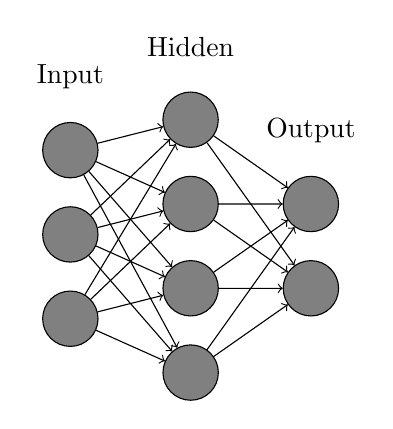
\begin{tikzpicture}[
    scale=1.2,
    basic/.style={draw,fill=gray,text badly centered,minimum width=2em},
    circ/.style={basic,circle,minimum width=2em},
]
    %inputs
    \node[circ] (i1) {};
    \node[circ,below of=i1,yshift=-0.2em] (i2) {};
    \node[circ,below of=i2,yshift=-0.2em] (i3) {};
    \node[above of=i1,yshift=-0.2em] {Input};

    \node[circ,right of=i1,xshift=1.5em,yshift=1.1em] (h1) {};
    \node[circ,below of=h1,yshift=-0.2em] (h2) {};
    \node[circ,below of=h2,yshift=-0.2em] (h3) {};
    \node[circ,below of=h3,yshift=-0.2em] (h4) {};
    \node[above of=h1,yshift=-0.2em] {Hidden};

    \node[circ,right of=h2,xshift=1.5em] (o1) {};
    \node[circ,right of=h3,xshift=1.5em] (o2) {};
    \node[above of=o1,yshift=-0.2em] {Output};

    \draw[->] (i1) -- (h1);
    \draw[->] (i1) -- (h2);
    \draw[->] (i1) -- (h3);
    \draw[->] (i1) -- (h4);
    \draw[->] (i2) -- (h1);
    \draw[->] (i2) -- (h2);
    \draw[->] (i2) -- (h3);
    \draw[->] (i2) -- (h4);
    \draw[->] (i3) -- (h1);
    \draw[->] (i3) -- (h2);
    \draw[->] (i3) -- (h3);
    \draw[->] (i3) -- (h4);

    \draw[->] (h1) -- (o1);
    \draw[->] (h1) -- (o2);
    \draw[->] (h2) -- (o1);
    \draw[->] (h2) -- (o2);
    \draw[->] (h3) -- (o1);
    \draw[->] (h3) -- (o2);
    \draw[->] (h4) -- (o1);
    \draw[->] (h4) -- (o2);
\end{tikzpicture} }
        \vspace{0.7em}
        \caption{A simple ANN}
        \label{subfig:simple_nn}
    \end{subfigure}
    
    \caption{(a) The basic structure of an artificial neuron and (b) a simple 3-layers feedforward ANN}
    \label{fig:artificial_neuron}
\end{figure}

The main unit composing an ANN is the artificial neuron.
The first artificial neuron was proposed by McCulloch and Pitts in 1943 \cite{McCulloch1943}.
Its generic structure is visible in figure \ref{subfig:artificial_neuron} and its output can be described by the following equation:
\begin{equation}
y = \varphi(\sum\limits_{i=1}^n w_ix_i + b)
\label{eqn:artificial_neuron}
\end{equation}
where $x_i$ are the input values, $w_i$ are the weights, $b$ is a bias term and $\varphi$ is the activation function.
In other words, the artificial neuron performs a linear combination of inputs $x$, weights $w$ and bias term $b$ and then applies a non-linearity using the function $\varphi$ to determine whether it should output a value based on the weighted sum of its inputs.
The correct values of weights that, given an input $x$, produce the desired output $y$ shall be found through learning.

The activation function shall be a differentiable function in order to apply common learning optimization methods, that are mentioned in \ref{sec:learning_process}.
The most used activation function is the rectified linear unit (ReLU) \cite{ramachandran2017searching} expressed by the equation:
\begin{equation}
    y = max(0, x)
    \label{eqn:relu}
\end{equation}

The network is usually formed by subsequent layers composed by multiple neurons, where the output of a layer is used as input of the following one; this structure is called feedforward ANN, since the flow of calculation is performed in a single forward direction forming an acyclic graph; other configurations are also possible that creates cycles like in recurrent neural networks \cite{lstm1997}.
An example of a 3-layers feedforward NN is depicted in figure \ref{subfig:simple_nn}. The first layer that receives external data is called \emph{input layer}, the last one that produces the results is called \emph{output layer}, all those between them are called \emph{hidden layers}.


\subsection{Learning Process} \label{sec:learning_process}
The goal of the learning process is to find the weights and bias values that allow to use the ANN to resolve a specific task whether it is a classification task, a regression or a different kind.
The task is represented as an optimization problem that consists of minimizing a loss function that measures the distance between the output calculated by the network $y_i$ and the expectation $\hat{y}_i$.
Most used loss functions are mean absolute error (MAE):
\begin{equation}
    MAE = \frac{1}{n} \sum\limits_{i=1}^n \mid y_i - \hat{y}_i \mid
    \label{eqn:mae}
\end{equation}
the mean squared error (MSE):
\begin{equation}
    MSE = \frac{1}{n} \sum\limits_{i=1}^n (y_i - \hat{y}_i)^2
    \label{eqn:mse}
\end{equation}
and for outputs that represent probability distributions cross entropy:
\begin{equation}
    H = - \sum\limits_{i=1}^n y_i \log \hat{y}_i
    \label{eqn:cross_entropy}
\end{equation}
and Kullback-Leibler divergence \cite{Kullback1951}:
\begin{equation}
    KLDiv = \sum_{i=1}^{N} \hat{y}_i log\frac{\hat{y}_i}{y{_i}}
    \label{eqn:kldiv}
\end{equation}

The process involves passing input training data through the network to calculate a prediction that is compared with the actual value, using the selected loss function; the gradient of the loss with respect to the weights and biases is then calculated using back-propagation \cite{rumelhart1986learning} layer by layer, starting from the output layer and moving backward to find how the weights and biases shall be changed to minimize the loss.
The network is then updated using an optimization strategy like stochastic gradient descent (SGD) or Adam \cite{kingma2014}, changing weights by little steps towards loss function decreasing direction, to find its minimum; the size of those steps is usually determined by a parameter called \emph{learning rate}.
The whole process is repeated for multiple iterations, or epochs, until the network prediction reliability is considered satisfactory enough or the network stops improving its performance.
It shall be considered that solutions to real-world problems are not trivial and the optimizer might not find the global minimum of the loss function, but instead get stuck in a local minima; to avoid this, learning rate and some other hyper-parameters can be tuned, but this requires many attempts and experience.


\section{Convolutional neural networks}
The usage of dense networks, i.e. ANNs composed by multiple fully-connected layers of neurons only, does not fit very well when the inputs are images: the high computational costs due to the size of the input layer and the lack of spatial correlation between pixels heavily limits the performance of ANN on images.
For this reason, convolutional neural networks (CNN) has been introduced.

Convolution is a mathematical operation that represents the amount of overlap of a function $g$ as it is shifted over another function $f$ \cite{wolfram_conv}.
Its discrete version where $f$ and $g$ are defined on integers set $\mathbb{Z}$ can be expressed as:
\begin{equation}
    (f * g)(n) = \sum\limits_{m=-\infty}^\infty f(m)g(n-m)
    \label{eqn:convolution}
\end{equation}

Convolution is widely used in image processing, it is performed adding to each pixel of an image the values of its neighbours weighted by the values of a matrix called kernel.
This operation transforms the original image and, based on the kernel used, can generate a blurred or a sharpen version of the image, can detect edges around objects or extract more complex features from the source.
In general, the kernel is used to represent or extract a specific feature of the image, e.g. lines, edges, circles, etc.
A kernel is a small, usually square, matrix specifically designed for a task, it is applied on the image starting from the first pixel on a corner and then shifted to cover the whole image; at each step the values of the pixel and its surrounding neighbours are multiplied by the corresponding values on the kernel and the results are then summed up to generate the output for the pixel.
An example of vertical edge detection kernel and its application is depicted in figure \ref{fig:convolution}.

\begin{figure}
    \centering
    \resizebox{0.8\textwidth}{!}{ 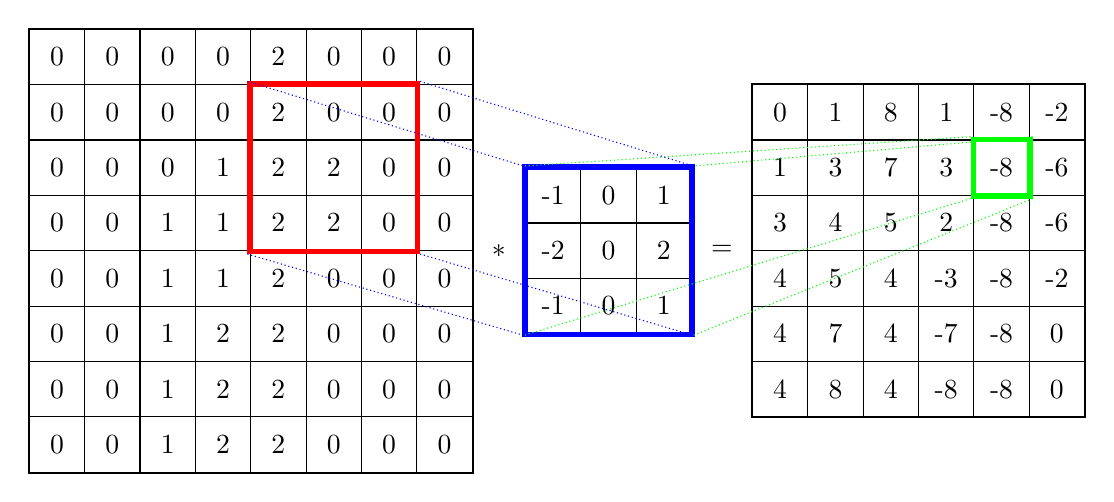
\begin{tikzpicture}[
    mmat/.style={
        matrix of nodes,
        nodes in empty cells,
        column sep=-\pgflinewidth/2,
        row sep=-\pgflinewidth/2,
        cells={nodes={draw,inner sep=0.5em,thin,minimum width=2em,minimum height=2em}},
        draw=#1,
        thick,
        inner sep=0pt
    },
    mmat/.default=black,
    node distance=0.3em
]
  \matrix[mmat](src){
    0 & 0 & 0 & 0 & 2 & 0 & 0 & 0 \\
    0 & 0 & 0 & 0 & 2 & 0 & 0 & 0 \\
    0 & 0 & 0 & 1 & 2 & 2 & 0 & 0 \\
    0 & 0 & 1 & 1 & 2 & 2 & 0 & 0 \\
    0 & 0 & 1 & 1 & 2 & 0 & 0 & 0 \\
    0 & 0 & 1 & 2 & 2 & 0 & 0 & 0 \\
    0 & 0 & 1 & 2 & 2 & 0 & 0 & 0 \\
    0 & 0 & 1 & 2 & 2 & 0 & 0 & 0 \\
  };
  \node[fit=(src-2-5)(src-4-7),inner sep=0pt,draw,red,line width=2pt](src_area){};

  \node[right=of src] (conv_op) {$*$};

  \matrix[mmat,right=of conv_op](kernel){
    -1 & 0 & 1 \\
    -2 & 0 & 2 \\
    -1 & 0 & 1 \\
  };
  \node[fit=(kernel-1-1)(kernel-3-3),inner sep=0pt,draw,blue,line width=2pt]{};

  \node[right=of kernel] (eq) {$=$};

  \matrix[mmat,right=of eq](dst){
    0 & 1 & 8 & 1 & -8 & -2 \\
    1 & 3 & 7 & 3 & -8 & -6 \\
    3 & 4 & 5 & 2 & -8 & -6 \\
    4 & 5 & 4 & -3 & -8 & -2 \\
    4 & 7 & 4 & -7 & -8 & 0 \\
    4 & 8 & 4 & -8 & -8 & 0 \\
  };
  \node[fit=(dst-2-5)(dst-2-5),inner sep=0pt,draw,green,line width=2pt](dst_pixel){};

  \foreach \Anchor in {south west,north west,south east,north east} {
    \draw[blue,densely dotted] (src_area.\Anchor) -- (kernel.\Anchor); 
    \draw[green,densely dotted] (dst_pixel.\Anchor) -- (kernel.\Anchor);
  }
\end{tikzpicture} }
    \caption{An example of convolution using a $3\times3$ kernel for vertical edge detection. High values in the output matrix on the right means a rising edge detected in the source image, low negative values a falling edge.}
    \label{fig:convolution}
\end{figure}

Since convolutions are capable to extract advanced features out of raw images they can be applied as a preprocessing step to prepare features for an ANN to perform a learning task.
In the past, preparing convolutional kernels was a manual operation that required advanced knowledge of image processing principles and on the specific task domain; often some well-known fixed kernels were used to extract common features like horizontal and vertical edges, flat areas, etc.
In 1989 LeCun et al. \cite{LeCun1989} had the intuition to combine convolutions and ANNs adding at the beginning of the network some layers composed by convolutional kernels which weights are learned by the network itself with back-propagation.
Using this approach network has the possibility to find out from data the best kernels to apply on images, often outperforming experts, to get good features on which fully connected layers can perform the desired task.
They invented convolutional neural networks.

It is possible to put in a row multiple convolutional layers in order to find more complex and specific features, combining simpler features from previous layers and increasing the receptive field, i.e. the portion of the image covered.
Each convolutional layer is usually followed by an activation function and by a pooling layer that performs downsampling of the image.
The idea behind downsampling is that high resolution is needed to detect first level features, but then precise position is not so important to compute following higher level features.

The architecture of a CNN can be usually splitted in two main sections: a convolutional feature extractor and a fully connected section that performs the final learning task, either it is classification, regression, segmentation or something else.
A good property of CNNs is also to have relatively few free parameters, that means less computational time and memory resources required, compared to a fully connected network of the same size.

Today CNNs are extensively applied with success to resolve learning tasks on many different domains not limited to image processing and computer vision, but including also video, audio and 3D image processing.


\section{Transfer learning}
One of the main problems of neural networks is that they are data hungry, meaning that they need a huge amount of data samples to be trained properly; without the latter, it is possible to incur in a phenomenon called overfitting, which happens when a model performs well on training data, but not on unseen data, i.e. it does not generalize.
Unfortunately, collecting and labeling a large amount of data to train a NN can be really expensive, time consuming and, sometimes, not possible at all.

The transfer learning approach can be used to address this problem \cite{ribani2019survey}.
The idea is that the knowledge learned by a model to solve a task can be somehow applied to a different learning problem, mitigating the limited amount of data available for the latter.
The two problems, source and target, may be different for the domain they apply to, for the task they want to resolve, or both.

The architecture of CNNs is well suited to perform transfer learning: the feature extractor of a CNN trained on a large, high quality dataset, should generate good features that are generic and describe well the source data, such features can be re-used to perform different tasks.
To train a CNN on a small dataset then, a common approach is to find a different large dataset sufficiently related to the target domain and train the model on it, even if the task could be different; this pre-trained network is then modified slightly, changing the fully connected layers to address the target task, and fine-tuning is performed executing some training iterations using the small dataset.
In some cases, when the two domains are really similar, and the target dataset is very small, can also be a good idea to freeze the convolutional layers during fine-tuning and train final layers only in order to avoid compromising the quality of the feature extractor due to overfitting.

This approach gives often better results compared to train a model from scratch on a small dataset, since the network have the chance to learn the structure and diversity of data from many different examples and usually generalize better on new data.
Transfer learning, anyway, can lead sometimes to worse performance, and this is called negative transfer.
This can happen, for example, when the domains are not related enough or there is a bias in the source domain.


\section{Knowledge distillation}
Knowledge distillation (KD) was introduced by \citeauthor{hinton2015distilling} \cite{hinton2015distilling} as a technique to transfer knowledge from one large NN, or an ensemble of networks, called teacher, to a smaller model called student.
The main purpose of this work was to compress complex models to reduce their size and computational requirements without losing performance.
In recent years many other studies have investigated KD \cite{gou2021knowledge}, going beyond its original purpose and exploring many different strategies.

The first component of a KD system is, of course, the knowledge.
\citeauthor{gou2021knowledge} \cite{gou2021knowledge} identify three categories of knowledge that can be transferred from a teacher to a student:
\begin{enumerate}
    \item \textbf{Response-based knowledge:} the knowledge is extracted directly from the output of the last layer of the network.
    To this category belongs the knowledge used by \citeauthor{hinton2015distilling} in \cite{hinton2015distilling}.
    The idea is to try to replicate the final prediction of the teacher optimizing the so-called distillation loss formulated as:
    \begin{equation}
        L_{resD}(z_t, z_s) = \mathcal{L}_R(z_t, z_s)
        \label{eqn:response_based_kd_loss}
    \end{equation}
    where $z_t$ and $z_s$ are respectively the logits of the teacher and the student and $\mathcal{L}_R$ is the divergence loss.
    In classification tasks, this is usually modified replacing the logits with class probabilities using a softmax function:
    \begin{equation}
        p(z_i, T) = \frac{e^{z_i/T}}{\sum_je^{z_j/T}}
        \label{eqn:softmax}
    \end{equation}
    where $z_i$ is the logits for the i-th class and $T$ is a factor, called temperature, to control the importance of each soft target: the higher the temperature the softer the probability distribution over classes.
    In this case the Kullback-Leibler divergence loss as stated in \ref{eqn:kldiv} is often used \cite{gou2021knowledge}.
    
    \item \textbf{Feature-based knowledge:} the output of intermediate layers is used as the knowledge to transfer.
    The aim in this case is to let both networks to extract same features out of data.
    To achieve this, an internal layer of both networks is selected and the student is pushed to produce the same features as the teacher at the selected layer.
    This type of knowledge is used for example in \cite{romero2014fitnets} and \cite{fini2022self}.
    The loss optimized is:
    \begin{equation}
        L_{feaD}(f_t(x), f_s(x)) = \mathcal{L}_F(\phi_t(f_t(x)), \phi_s(f_s(x)))
        \label{eqn:feature_based_kd_loss}
    \end{equation}
    where $f_t(x)$ and $f_s(x)$ are respectively the feature maps of the intermediate layers of the teacher and the student and $\phi_t$, $\phi_s$ are functions applied when the maps are not in the same shape.
    Usually $l_2$-norm, $l_1$-norm and cross-entropy are used as $\mathcal{L}_F$.
    
    \item \textbf{Relation-based knowledge:} the knowledge is not taken directly from a network layer of the teacher, but the relationship between different layers is used.
    This is the most complicated type of knowledge to transfer.
    The loss can be formulated as:
    \begin{equation}
        L_{relD}(f_t, f_s) = \mathcal{L}_{R^1}(\Psi_t(\hat{f}_t, \check{f}_t), \Psi_s(\hat{f}_s, \check{f}_s))
        \label{eqn:relation_based_kd_loss}
    \end{equation}
    where $f_t$ and $f_s$ are respectively feature maps of teacher and student, $\hat{f}_t$ and $\check{f}_t$ are two selected maps from the teacher and $\hat{f}_s$ and $\check{f}_s$ from the student and $\Psi_t$, $\Psi_s$ are similarity functions for pairs of maps and $\mathcal{L}_{R^1}$ is the distance between them.
\end{enumerate}

Once the type of knowledge is chosen, another perspective to take into account for KD is the distillation scheme, i.e. when the teacher and the student are trained, if simultaneously or not.
We can identify three possible schemes:
\begin{enumerate}
    \item \textbf{Offline distillation:} the teacher is pre-trained and then frozen during distillation; this is the simplest approach used in \cite{hinton2015distilling}.
    \item \textbf{Online distillation:} the teacher and the student are trained together; this scenario is especially suited for collaborative \cite{zhang2018deep} and/or adversarial \cite{zhang2021adversarial} distillations.
    \item \textbf{Self-distillation:} the same network is used as teacher and as student \cite{zhang2019your}.
\end{enumerate}

Another fundamental aspect of this methodology is the choice of both teacher and student network architectures; if the size and the capacity gap between the two is too large, the distillation could be degraded or not beneficial at all.
The student network is usually chosen to be a simplified or quantized version of the teacher or even a network with the same structure of the teacher \cite{gou2021knowledge}; there is not a catch-all recipe to design the best architecture for KD, but it shall be found specifically for each case

The last component of KD is the algorithm used to transfer the knowledge; it can be the simple match of teacher and student knowledge or a more sophisticated method such as:
\begin{itemize}
    \item \textbf{Adversarial distillation:} inspired by concepts from generative adversarial networks \cite{belagiannis2018adversarial}.
    \item \textbf{Multi-teacher distillation:} that uses multiple teachers for the same student \cite{hinton2015distilling}.
    \item \textbf{Multi-modal distillation:} where teacher and student are trained on different modalities of the same subject \cite{zhang2023distilling}, for example optical and depth images, that can help to mitigate limited amount of data in the student modality.
\end{itemize}

\chapter{Dataset}\label{sec:dataset}

For the purposes of this project, we used a dataset that allows us to associate a CT scan and an X-ray of the same patient acquired with a relatively short time gap; this let us to be reasonably confident about the correlation of information present in these two exams.
Comparing our dataset to that used by \citeauthor{zhang2023distilling} in \cite{zhang2023distilling} that develop a similar KD approach, we can note that our data association is more conservative and we suppose should be more reliable: their pairing of data from different modalities is performed matching samples belonging to the same class, whereas we are pairing data from the same patient.

In particular, our dataset has been provided by \emph{Città della Salute e della Scienza di Torino} hospital and is composed by 491 paired frontal CXRs and relative CT scans of the same patients, labelled by experts with the CAC score.
Beside the paired samples, we exploited also 112 additional CXRs without their respective CT scans, that we use to validate our results during the testing phase.

The paired scans has been acquired at 39 days apart on average, with values ranging from both analysis performed on the same day up to about 3 years, median value is 12 days.
Time gap between exams is important for the reliability of labelling considering that CAC scoring is performed on CTs.
Based on the order in which the tests are performed and on the class the patient belongs to, we can divide the possible cases into four possible scenario:
\begin{itemize}
    \item CT before CXR on negative patient: if long time occurs between the two exams the patient could turn to positive in the meantime and classification on CXR is compromised.
    \item CT before CXR on positive patient: since no known pharmacological methods can lead to CAC regression \cite{Czaja-Ziolkowska2022-pd} we are sure that when the CXR is performed the CAC is still positive and its value may only be greater or equal than before. 
    \item CT after CXR on negative patient: for the same reason as before, the patient was certainly already negative when CXR was performed.
    \item CT after CXR on positive patient: in this case it is possible that the patient was negative when CXR was performed and became positive during the time elapsed between exams.
\end{itemize}
However, the time gap between our paired samples is generally short enough to give us a good confidence about reliability of the classification, with low probability that class of the patient can change between the two exams.

In the following section we describe the image we have at our disposal, whereas in \ref{sec:dataset_distribution} we perform an accurate statistical analysis of our dataset, in order to have clear in mind what kind of data we are using.


\section{Image types: CT scans and CXR}

\subsection{CT Scans}

The 491 CT scans has been acquired by 9 different devices, using different protocols, and focusing on different portion of the body.
Indeed, some of them focus on the cardiac area only, with a very high resolution, some have a slightly larger field of view, including the whole body width, and a lower resolution.
Slice thickness is between 0.6mm and 3mm with an average of 1.3mm and a median and mode of 1.25mm.
All scans are composed by a variable number of slices between 123 and 1100 of the same size of $512 \times 512$ voxels, with only 2 exceptions that are $768 \times 768$.
Despite their differences, they are all suitable for CAC scoring performed by experts, and we assume that a properly trained NN could effectively perform CAC detection on them.
Some examples of different types of CT scans available in our dataset are depicted in figure \ref{fig:ct_example}.

\begin{figure}
    \centering
    \begin{subfigure}[b]{0.3\textwidth}
        \resizebox{\textwidth}{!}{ \includegraphics{ct_example_large} }
        \caption{}
        \label{subfig:ct_example_large}
    \end{subfigure}\hspace{1em}
    \begin{subfigure}[b]{0.3\textwidth}
        \resizebox{\textwidth}{!}{ \includegraphics{ct_example_medium} }
        \caption{}
        \label{subfig:ct_example_medium}
    \end{subfigure}\hspace{1em}
    \begin{subfigure}[b]{0.3\textwidth}
        \resizebox{\textwidth}{!}{ \includegraphics{ct_example_small} }
        \caption{}
        \label{subfig:ct_example_small}
    \end{subfigure}
    
    \caption{Some slices in axial projection at increasing depths of 3 CT scans acquired using different protocols and different fields of view. Images from our dataset.}
    \label{fig:ct_example}
\end{figure}


\subsection{CXR}

Differently from CTs, the 603 CXRs have been acquired by more than 20 different devices in different projections, 408 of them are marked as posteroanterior views; this projection is preferable since the heart is generally clearly visible on it.
The remaining images are anteroposterior, where the image is often blurred and heart shape is deformed.
For 44 patients also a lateral CXR is available, but those images are not considered for this work since visibility of the heart is limited and the number of samples is very low.
Main differences between the three possible CXR projections can be observed in some examples depicted in figure \ref{fig:cxr_example}.
The size of the images are varying, from a minimum of $1733\times1715$ to a maximum of $4020\times4892$, presented in different proportions.

This dataset extends the one used by \cite{iodice_2022}, including all the CXRs used in that work.

\begin{figure}
    \centering
    \begin{subfigure}[b]{0.3\textwidth}
        \resizebox{\textwidth}{!}{ \includegraphics{cxr_example_pa} }
        \caption{}
        \label{subfig:cxr_example_pa}
    \end{subfigure}\hspace{1em}
    \begin{subfigure}[b]{0.3\textwidth}
        \resizebox{\textwidth}{!}{ \includegraphics{cxr_example_ap} }
        \caption{}
        \label{subfig:cxr_example_ap}
    \end{subfigure}\hspace{1em}
    \begin{subfigure}[b]{0.3\textwidth}
        \resizebox{\textwidth}{!}{ \includegraphics{cxr_example_lat} }
        \caption{}
        \label{subfig:cxr_example_lat}
    \end{subfigure}
    
    \caption{Examples of (a) posteroanterior, (b) anteroposterior and (c) lateral X-rays.
             Images from our dataset.}
    \label{fig:cxr_example}
\end{figure}


\section{Statistical analysis of the clinical data}\label{sec:dataset_distribution}

In this section we analyze the clinical data (i.e. age, gender, CAC distribution) associated to our dataset, that is composed by patients aged between 3 and 93 years, with an average age of 62 years.
Distribution of patients by age is depicted in figure \ref{subfig:dataset_patients_by_age}; the most represented class is that of people in their sixties and over 60\% of the dataset is composed by people over this age.
From figure \ref{subfig:dataset_cac_avg_by_age}, we can see that all patients below 30 years are negatives while people above 60 years have, on average, a CAC score greater than 1000.
Generally we can see that CAC score increases with age, with the only exception of the class of people above age of 90 that has, however, very few samples.

Figure \ref{subfig:dataset_patients_by_cac} shows distribution of patients by CAC score grouped by risk categories of table \ref{tab:agatston-risk}, with 39\% of patients in the very low risk category, i.e. negative class in our task with no calcium detected, and 61\% with a CAC score greater that zero; of them the majority is in the very high risk category.
The low, intermediate and high risk classes are less represented in our dataset and those likely contain patients that are presumably harder to classify; this is an additional complication to solve our classification task, since indeed more samples of those classes could be helpful to train a better classifier.
The dataset is also biased towards male gender, that represents 60\% of patients,  67\% of them have positive value of CAC, against 51\% of positives in the female subset, as shown on figure \ref{subfig:dataset_cac_by_gender}.

An overall summary of class distribution across gender and age is shown in table \ref{tab:pos_neg_distribution}.
Distribution of our dataset is consistent with other studies, showing that the likelihood of developing CAC increases with age and is related to gender \cite{Czaja-Ziolkowska2022-pd}.

\begin{figure}
    \centering
    \begin{subfigure}[b]{0.45\textwidth}
        \resizebox{\textwidth}{\textwidth}{ \begin{tikzpicture}
    \begin{axis}[
        name=age_plot,height=9cm,width=9cm,
        % title={Age distribution},
        ybar,
        ymin=0,ylabel={Patients},
        xmin=0,xmax=100,xlabel={Age} 
    ]
        \addplot +[
            hist={
                bins=10,
                data min=0,
                data max=100
            }   
        ] table [y index=0] {data/age.csv};
    \end{axis}
\end{tikzpicture}
 }
        \caption{}
        \label{subfig:dataset_patients_by_age}
        \vspace*{3em}
    \end{subfigure}
    \begin{subfigure}[b]{0.45\textwidth}
        \resizebox{\textwidth}{\textwidth}{ 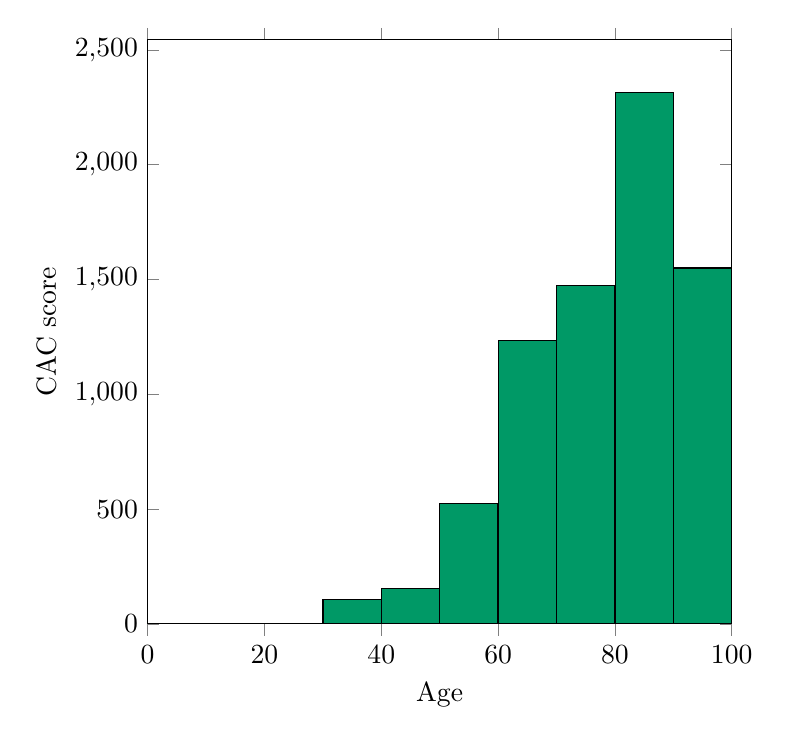
\begin{tikzpicture}
    \begin{axis}[
        name=cac_avg_by_age,height=9cm,width=9cm,
        ybar,
        ymin=0,ylabel={CAC score},
        xmin=0,xmax=100,xlabel={Age},
        bar width=21pt,
    ]
        \addplot[fill=green!60!blue] coordinates {
            (5,0)
            (15,0)
            (25,0)
            (35,107)
            (45,155)
            (55,525)
            (65,1234)
            (75,1474)
            (85,2313)
            (95,1550)
        };
    \end{axis}
\end{tikzpicture}
 }
        \caption{}
        \label{subfig:dataset_cac_avg_by_age}
        \vspace*{3em}
    \end{subfigure}

    \begin{subfigure}[b]{0.45\textwidth}
        \resizebox{\textwidth}{\textwidth}{ \begin{tikzpicture}
    \begin{axis}[
        name=cac_plot,at={($(age_plot.east)+(2cm,0)$)},anchor=west,height=9cm,width=9cm,
        % title={CAC score distribution},
        ybar,
        symbolic x coords={0, 1-10, 11-100, 101-400, >400},
        ymin=0,ylabel={Patients},
        xmin=0,xtick=data,xlabel={CAC score},
        bar width=30pt,
        enlarge x limits=0.1,
        % nodes near coords={\pgfmathprintnumber\pgfplotspointmeta} % put value on bar top
    ]
        \addplot[fill=orange!70] coordinates {
            (0,235)
            (1-10,10)
            (11-100,55)
            (101-400,64)
            (>400,239)
        };
    \end{axis}
\end{tikzpicture}
 }
        \caption{}
        \label{subfig:dataset_patients_by_cac}
    \end{subfigure}
    \begin{subfigure}[b]{0.45\textwidth}
        \resizebox{\textwidth}{\textwidth}{ 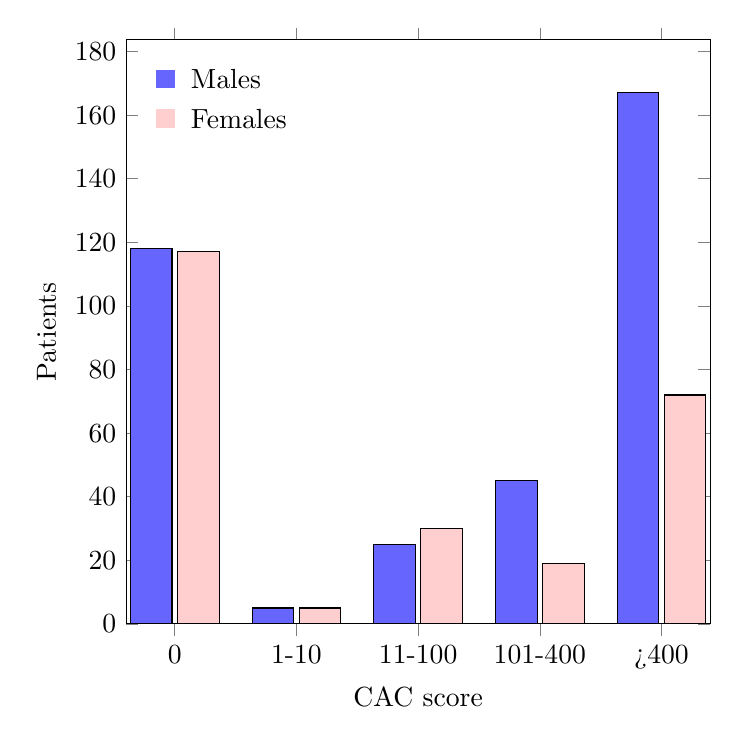
\begin{tikzpicture}
    \begin{axis}[
        name=cac_by_gender,height=9cm,width=9cm,
        % title={CAC score by gender distribution},
        ybar,
        symbolic x coords={0, 1-10, 11-100, 101-400, >400},
        ymin=0,ylabel={Patients},
        xmin=0,xtick=data,xlabel={CAC score},
        bar width=15pt,
        enlarge x limits=0.1,
        % nodes near coords={\pgfmathprintnumber\pgfplotspointmeta} % put value on bar top
    ]
        \addplot[fill=blue!60] coordinates {
            (0,118)
            (1-10,5)
            (11-100,25)
            (101-400,45)
            (>400,167)
        };
        \addplot[fill=pink!75] coordinates {
            (0,117)
            (1-10,5)
            (11-100,30)
            (101-400,19)
            (>400,72)
        };
    \end{axis}
    \node[fill=blue!60,xshift=0.5cm,yshift=-0.5cm] at (cac_by_gender.north west) (male) {};
    \node[right of=male,anchor=west,xshift=-0.8cm] {Males};
    \node[fill=pink!75,below of=male,yshift=0.5cm] (female) {};
    \node[right of=female,anchor=west,xshift=-0.8cm] {Females};
\end{tikzpicture}
 }
        \caption{}
        \label{subfig:dataset_cac_by_gender}
    \end{subfigure}\hspace{1em}

    \caption{(a) Dataset distribution of patients by age, (b) CAC average by age, (c) patients by CAC score grouped by risk category, (d) CAC distribution by gender and risk category.}
    \label{fig:dataset_distribution}
\end{figure}

\begin{table}
    \centering
    \begin{tabular}{|l|r c|r c|c|}
        \hline
        & \multicolumn{2}{c|}{\textbf{Negatives}} & \multicolumn{2}{c|}{\textbf{Positives}} & \textbf{TOTAL} \\
        \hline
        Male    & 118 & (32,8\%) & 242 & (67,2\%) & 360 \\
        Female  & 117 & (48,1\%) & 126 & (51,9\%) & 243 \\
        \hline
        Age 0-9   &   1 &  (100\%) &   0 &    (0\%) &   1 \\
        Age 10-19 &  13 &  (100\%) &   0 &    (0\%) &  13 \\
        Age 20-29 &  28 &  (100\%) &   0 &    (0\%) &  28 \\
        Age 30-39 &  28 & (96,6\%) &   1 &  (3,4\%) &  29 \\
        Age 40-49 &  47 & (79,7\%) &  12 & (20,3\%) &  59 \\
        Age 50-59 &  54 & (52,9\%) &  48 & (47,1\%) & 102 \\
        Age 60-69 &  42 & (29,0\%) & 103 & (71,0\%) & 145 \\
        Age 70-79 &  13 &  (9,8\%) & 120 & (90,2\%) & 133 \\
        Age 80-89 &   8 & (10,0\%) &  72 & (90,0\%) &  80 \\
        Age 90+   &   1 &  (7,7\%) &  12 & (92,3\%) &  13 \\
        \hline
        \hline
        Training set   & 164 & (40.3\%) & 243 & (59.7\%) &    407 \\
        Test set (CT)  &  32 & (38.1\%) &  52 & (61.9\%) &     84 \\
        Test set (CXR) &  71 & (36.2\%) & 125 & (63.8\%) & 84+112 \\
        \hline
        \hline
        ALL       & 235 & (39,0\%) & 368 & (61,0\%) & 603 \\
        \hline
    \end{tabular}
    \caption{Distribution of data between positives and negatives classes}
    \label{tab:pos_neg_distribution}
\end{table}

Throughout this work, the dataset has been split in two parts to compose a training set and a test set with approximately same class distribution.
From the entire set of patients with both a CXR and a CT scan, we removed randomly 84 samples to compose the test set, the remaining have been used as the training set.
Furthermore, as mentioned at the beginning of this chapter, all 112 CXRs that do not have a paired CT scan have been included in the test set of the experiments that use X-ray images as inputs, for a total of 196 samples.

\chapter{Method}\label{sec:method}
\begin{figure}
    \centering
    \resizebox{0.8\textwidth}{!}{ \includegraphics{method} }
    \caption{An overview of the method applied: at first some models are trained on CT scans, then knowledge is distilled from the CT classifier
    to a CXR classifier.}
    \label{fig:method}
\end{figure}

The goal of our work is to train an artificial neural network that can detect if coronary calcium is present or not in a patient from their CXR, to achieve this, we structured the work as a binary classification learning problem.

Due to the inherent complexity of the task and the limited amount of data available, the training has been performed using multi-modal knowledge distillation.
Leveraging peculiarities of our dataset, we used the CT scans to resolve the same classification task, but on a modality in which the problem is actually simpler and already addressed in many works in literature \cite{vanvelzen2021ai}.
Then we exploited the models trained on CTs as teachers to drive the training of a student network that works on the paired CXRs of the same patients.
Since a network trained for a complex task with limited data will likely suffer of overfitting, the idea is to limit it pushing the student to extract better and more generic feature maps while trying to solve the problem and in the meantime mimic behaviour of the teacher which have better generalization capabilities.

An overview of the method is shown in figure \ref{fig:method}.

The rest of this chapter is composed by two sections: at first in \ref{sec:detecting_calcium_on_ct} all the steps for calcium detection on CT scans are presented, including both data preprocessing and model architecture, then on section \ref{sec:detecting_calcium_on_cxr} we describe all the techniques we implemented for detection on CXRs.


\section{Detecting calcium on CT}\label{sec:detecting_calcium_on_ct}

In the last years many methods have been applied to CAC score estimation exploiting CT scans, for example those proposed by \citeauthor{Wolterink2015-ii} \cite{Wolterink2015-ii}, \citeauthor{Lessmann_2018} \cite{Lessmann_2018}, \citeauthor{Cano-Espinosa2018-gm} \cite{Cano-Espinosa2018-gm} and \citeauthor{de_Vos_2019} \cite{de_Vos_2019}, that have been briefly described in section \ref{sec:related_works}.
The availability of many studies on this topic shows that the problem is well known and many techniques have already been explored, sometimes with very good results: \citeauthor{de_Vos_2019} \cite{de_Vos_2019} for example achieved 93\% accuracy on risk category classification.
Interest in the field is also supported by image analysis challenges on this task, such as the \emph{orCaScore} \cite{wolterink2016evaluation} aiming at benchmarking performance of proposed methods.
Test sets contained in challenges typically provide images acquired with a multitude of diverse devices and protocols proving generalization effectiveness and indicating great potential for application in clinical practice \cite{vanvelzen2021ai}.

Many studies are based on 2D convolutional networks working on a single slice of the CT at a time; this is the case, for example, for methods from \citeauthor{Lessmann_2018} \cite{Lessmann_2018} and \citeauthor{de_Vos_2019} \cite{de_Vos_2019}.
This choice is possible whenever the dataset provides a CAC score label for each slice, meaning that, instead of using each CT scan as a single sample, hundreds of images are available for each patient with a single scan, dramatically increasing the size of the dataset.
On the contrary, due to the characteristics of our dataset that provides a single label for each CT, we propose the usage of 3D CNNs working on the whole CT scan.
This introduces additional challenges due to the smaller number of samples and higher computational requirements compared to 2D convolution approach.
In comparison with methods cited above we shall consider, however, that our problem is limited to a classification learning problem with only two classes: positives, with CAC > 0, and negatives, with CAC = 0; then some of the complexity of using 3D convolutions is already mitigated by the simpler task, whereas computational effort is reduced with preprocessing and crop of images as described in next section.


\subsection{Preprocessing of CT}

In order to level out some of the possible differences in images related to the devices used for acquisition and to the different protocols, that could have a negative impact on training, we applied a common preprocessing to them.
At first all the CT scans has been clipped between -1000 and 1000 HU, thus removing spike values below air or above bones density, and then rescaled in range $[-1; 1]$.

Furthermore, since the size of a CT scan is directly related to the amount of memory and time required for its analysis, we identified a method to reduce their size without affecting the quality of data.
The average size of a CT scan in our dataset is $300\times512\times512$ (depth $\times$ height $\times$ width).
It is a very large size that would easily lead to an explosion of parameters in the model, quickly exceeding memory size of a modern powerful GPU.
Also worth to be considered that most of the volume is not involved in CAC score at all; even on CT scans limited to the cardiac area, only few voxels in the image represent calcium lesions in the coronary arteries.
Remove all areas that surely do not contain information about coronary calcium could help also to avoid that spurious correlations between CAC and unrelated characteristics of other body parts could affect training.
The idea is then to reduce the size of the image removing everything that is not included in the near surrounding of the myocardium.
In the next section we describe the steps applied for heart segmentation and crop of the images.


\subsubsection{Cardiac area extraction}

CT scan segmentation is a field that has received a lot of interest and effort, since is often the first step to deal with in order to resolve more complex tasks.
The main challenge to perform segmentation with NN is to have a wide dataset and, for supervised learning, to have high quality annotations of organs and anatomical structures of the body.

An open dataset for heart segmentation has been found in Kaggle platform \cite{kaggle_heart_dataset}.
The training set of this dataset is composed by more than 2500 slices from 19 patients; for each image a corresponding mask of the heart shape is available.
The test set do not include the annotated masks and was not used, to replace it 4 patients from the train set has been excluded during training.
Due to the characteristic of this dataset the model shall work on 2D slices.

We used a library implemented by \citeauthor{Iakubovskii:2019} \cite{Iakubovskii:2019} to easily load well-known models that are at the state of the art for image segmentation.
Two different models have been compared to perform heart segmentation on Kaggle dataset: U-Net \cite{ronneberger2015u} and FPN \cite{lin2017feature}.
These are very similar models that use multiple convolutional and pooling layers to downsample and extract features, then use again convolutions combined with upsampling layers to build a segmentation mask.
The characteristic of these networks is that the features extracted at each downsampling layer are concatenated with each corresponding upsampling step.
The structures of the networks are depicted in figures \ref{fig:unet} and \ref{fig:fpn}.

\begin{figure}
    \centering
    \resizebox{0.9\textwidth}{!}{ \includegraphics{unet} }
    \caption{U-Net architecture. Image from \cite{ronneberger2015u}}
    \label{fig:unet}
\end{figure}
\begin{figure}
    \centering
    \resizebox{0.6\textwidth}{!}{ \includegraphics{fpn} }
    \caption{FPN architecture for object segmentation. Image from \cite{lin2017feature}}
    \label{fig:fpn}
\end{figure}

For both models we used a version of the network pre-trained on ImageNet dataset \cite{imagenet_cvpr09} and we evaluated the performance exploiting intersection over union (IoU) score.
Both networks have been trained for 50 epochs on the 15 patients left of the training set.
They achieved very similar results on the test set with a IoU of 0.932 for the U-Net and a IoU of 0.933 for the FPN.
For its slightly better result, predictions from the FPN network were used for the heart crop.

\begin{figure}
    \centering
    \begin{subfigure}[c]{0.3\textwidth}
        \resizebox{\textwidth}{!}{ \includegraphics{heart_segmentation_axial} }
        \caption{}
        \label{subfig:heart_segmentation_axial}
    \end{subfigure}\hspace{1em}
    \begin{subfigure}[c]{0.3\textwidth}
        \resizebox{\textwidth}{!}{ \includegraphics{heart_segmentation_coronal} }
        \caption{}
        \label{subfig:heart_segmentation_coronal}
    \end{subfigure}\hspace{1em}
    \begin{subfigure}[c]{0.3\textwidth}
        \resizebox{\textwidth}{!}{ \includegraphics{heart_segmentation_sagittal} }
        \caption{}
        \label{subfig:heart_segmentation_sagittal}
    \end{subfigure}
    
    \caption{Heart segmentation view on (a) axial, (b) coronal and (c) sagittal projections of a CT scan.
             The white area represent the mask predicted by FPN segmentation model.}
    \label{fig:heart_segmentation}
\end{figure}

FPN predictions of heart shape on each slice produce on the CT scan a result that is visible in figure \ref{fig:heart_segmentation}.
The heart seems very well identified even if the areas found by the model are not perfectly aligned on different slices.
To avoid that some false positives distant from the heart could affect the crop, the mask is refined limiting it to the largest connected component only.

A crop of size $150\times220\times280$ is then extracted from the CT scan at the position of the largest connected component found in the mask, downscaling the image to fit the size if required.
The size is determined empirically, with the requirement to fit at least 90\% of the crop areas extracted from our dataset without downscaling. 

For each refined mask, the convex hull including the shape of the heart is calculated using \emph{Quickhull} algorithm \cite{barber1996quickhull}: every voxel out of the hull is then removed setting it to a value of -1000 HU.

The final result of data preparation is shown in figure \ref{fig:heart_crop}.

\begin{figure}
    \centering
    \begin{subfigure}[c]{0.3\textwidth}
        \resizebox{\textwidth}{!}{ \includegraphics{heart_crop_axial} }
        \caption{}
        \label{subfig:heart_crop_axial}
    \end{subfigure}\hspace{1em}
    \begin{subfigure}[c]{0.3\textwidth}
        \resizebox{\textwidth}{!}{ \includegraphics{heart_crop_coronal} }
        \caption{}
        \label{subfig:heart_crop_coronal}
    \end{subfigure}\hspace{1em}
    \begin{subfigure}[c]{0.3\textwidth}
        \resizebox{\textwidth}{!}{ \includegraphics{heart_crop_sagittal} }
        \caption{}
        \label{subfig:heart_crop_sagittal}
    \end{subfigure}
    
    \caption{Final result of data preparation steps view on (a) axial, (b) coronal and (c) sagittal projections of a CT scan.}
    \label{fig:heart_crop}
\end{figure}


\subsection{Architecture of teacher models}

We developed two different models for calcium classification on CT scans.
These are used as teachers in the knowledge distillation training to try to improve performance of CXR classification and therefore is required they perform better than their CXR counterpart.
The two models are built with different structures and complexity in order to verify also impact of model architecture on knowledge distillation; they are:
\begin{enumerate}
    \item \textbf{Simple CT classifier (SimpleCT):} a naive implementation of a CNN with some consecutive convolutional layers followed by a fully
    connected classifier
    \item \textbf{Retina CT classifier (RetinaCT):} a more advanced network derived from RetinaNet \cite{lin2017focal}
\end{enumerate}

In the following paragraphs we detail the characteristics of SimpleCT and RetinaCT, respectively.  


\subsubsection{SimpleCT}
SimpleCT model is composed by 4 convolutional layers followed by an adaptive average pooling and a fully connected classifier.
Each convolutional layer is composed by 3D convolution, ReLU activation, max pooling and batch normalization.
Batch normalization helps to regularize the network and allows to use higher learning rates accelerating training \cite{ioffe2015batch}.
Features extracted by convolutional layers are then flattened by an adaptive average pooling layer that outputs a single average value for each input channel; the flat feature vector is then used to feed a classifier composed by multiple layers of fully connected neurons followed by batch normalization and ReLU activations.
The complete architecture is:

\begin{longtable}{l|l}
    \hline
    \multirow{4}{*}{\textbf{Conv1}} & 3D Convolution (kernel $7\times7\times7$, Stride $2\times2\times1$, 64 out channels) \\
    & ReLU \\
    & Max pooling (kernel $2\times2\times2$) \\
    & Batch normalization \\
    \hline
    \multirow{4}{*}{\textbf{Conv2}} & 3D Convolution (kernel $3\times3\times3$, Stride $1\times1\times1$, 128 out channels) \\
    & ReLU \\
    & Max pooling (kernel $2\times2\times2$) \\
    & Batch normalization \\
    \hline
    \multirow{4}{*}{\textbf{Conv3}} & 3D Convolution (kernel $3\times3\times3$, Stride $1\times1\times1$, 256 out channels) \\
    & ReLU \\
    & Max pooling (kernel $2\times2\times2$) \\
    & Batch normalization \\
    \hline
    \multirow{4}{*}{\textbf{Conv4}} & 3D Convolution (kernel $3\times3\times3$, Stride $1\times1\times1$, 512 out channels) \\
    & ReLU \\
    & Max pooling (kernel $2\times2\times2$) \\
    & Batch normalization \\
    \hline
    \textbf{Adaptavg} & 3D Adaptive average pooling \\
    \hline
    \multirow{3}{*}{\textbf{FC1}} & Linear (512 inputs, 128 outputs) \\
    & Batch normalization \\
    & ReLU \\
    \hline
    \multirow{3}{*}{\textbf{FC2}} & Linear (128 inputs, 32 outputs) \\
    & Batch normalization \\
    & ReLU \\
    \hline
    \textbf{FC3} & Linear (32 inputs, 2 outputs) \\
    \hline
\end{longtable}

\begin{figure}[h]
    \centering
    \resizebox{0.5\textwidth}{!}{ \includegraphics{simple_ct_architecture} }
    \caption{SimpleCT model architecture}
    \label{fig:simple_ct_architecture}
\end{figure}


\subsubsection{RetinaCT}
RetinaCT model is derived from RetinaNet \cite{lin2017focal}, a CNN model for object detection composed by a backbone FPN and two subnets, for object classification and bounding box regression respectively.
In this work we exploited a version of RetinaNet from MonAI project \cite{MONAI} pre-trained on the well-known LUNA16 \cite{luna16} dataset for lung nodules detection. 

From the pre-trained RetinaNet we removed both subnets and the deconvolutional section of the FPN, actually keeping only the basic ResNet \cite{he2016deep} feature extractor.
ResNet is a CNN with additional shortcut connections that add outputs of a convolutional layer to the outputs of a following layer.
The extracted ResNet is then used as the first block of RetinaCT, followed by an adaptive average pooling and a 3-layers fully connected classifier with the same shape as that used in SimpleCT network.

Compared to the previous structure, RetinaCT is more complex, with 23 convolutional layers and shortcut connections, for a total of 2,929,250 training parameters; on the contrary, SimpleCT, despite its simple architecture, is composed by 4,739,874 parameters.

\begin{figure}
    \centering
    \resizebox{0.9\textwidth}{!}{ \includegraphics{retinanet_architecture} }
    \caption{RetinaNet architecture. Image from \cite{lin2017focal}}
    \label{fig:retina_net_architecture}
\end{figure}


\subsection{Training on CT}
Both models described in the previous section have been optimized using the cross entropy loss formulated as the equation \ref{eqn:cross_entropy}.
The output logits of the classifier are converted into a probability distribution applying a softmax function formulated as \ref{eqn:softmax}.

Optimization method used is Adam \cite{kingma2014} configured with a learning rate of 0.01, halving it every 20 epochs.

We tried to avoid overfitting by adding also a l2-regularization term to the loss function as follows:
\begin{equation}
    Loss_{l2reg} = Loss(y_i, \hat{y}_i) + \lambda\sum\limits_{i=1}^n w_i^2
    \label{eqn:l2_regularization}
\end{equation}
where $y_i$ and $\hat{y}_i$ are the outputs of the network and the expected results respectively, $w_i$ are the trainable weights of the model, and $\lambda$ is a parameter controlling the importance of the l2 term, which has been set to $10^{-4}$.

In some experiments involving RetinaCT, the first convolutional layers of the pre-trained encoder has been freezed.
This transfer learning approach helps to avoid overfitting that can occur using a high-capacity network as RetinaCT with a small dataset as in our case and can be applied whenever the features extracted are of good quality and source and target domains are similar enough.

Tuning of hyper-parameters has been performed using 5-fold cross validation as reference for evaluation of training performance with special attention to overfitting.
Cross validation has also been used as confirmation of results since our defined test set is quite small and could suffer of undetected biases.
When all parameters are chosen the training is then repeated on the whole training set and generated model performance is finally verified on the test set.


\section{Detecting calcium on CXR}\label{sec:detecting_calcium_on_cxr}

CAC estimation from CXR is considered an hard task if even possible: calcium lesions can be really hard to detect since partially hidden by bones or blended with other tissues due to the 2D projection that is impressed on the X-ray image.
As discussed in section \ref{sec:related_works}, there are very few works trying to estimate CAC score or divides patients on risk categories, with promising results that are, however, still too far from quality required for clinical application.
The contribute of this work is to explore multi-modal knowledge distillation to understand if knowledge learned from CT scans can improve state-of-the-art performance of CAC classification on CXR.
For this purpose we use models described in the previous sections trained on CT scans as teachers to drive training of NNs that use only CXRs as input.


\subsection{Preprocessing of CXR}

We decided to apply to CXRs the same data preprocessing as used in \cite{iodice_2022} since our dataset is an extension of the one used in that work, in order to be able to better compare results.
At first, X-ray images in dicom format are loaded using SimpleITK library \cite{lowekamp2013design} that automatically transforms them to MONOCHROME2 photometric interpretation, if not already in that format: it means that dark areas are used to represent low density tissues, while lighter areas are the high density regions; this is required since some devices generate images using the opposite convention.
Then windowing is applied based on values contained in the metadata.
After that histogram equalization is performed to improve contrast and image is converted to 8 bits per pixel (bpp) to align different resolutions used, varying from 10 to 16 bpp.

Images are then resized to $1248\times1248$ pixels and a center crop of size $1024\times1024$ is extracted.
This crop has been manually verified to not remove any portion of the cardiac area.
Finally pixel values are rescaled in range $[0, 1]$ and normalization of the image is performed, replacing each value $x$ with the formula:
\begin{equation}
    x' = \frac{x - \mu}{\sigma}
    \label{eqn:normalization}
\end{equation}
using $\mu=0.5024$ and $\sigma=0.2898$ calculated as mean and standard deviation of CheXpert dataset, considering it as more representative of radiographs due to its very large size and since some reference models we use are pre-trained on that dataset.


\subsection{Architecture of student model}

The model chosen as the student of the knowledge distillation has a simple architecture, derived directly from SimpleCT model used for classification on CT scans.
The goal is to use a network that is similar enough to the teacher to take advantage of the common structures and easily perform response-based and feature-based KD.

The model is called SimpleCXR and is an adaptation of SimpleCT network replacing each 3D layer with 2D equivalent.
The architecture is then:

\begin{longtable}{l|l}
    \hline
    \multirow{4}{*}{\textbf{Conv1}} & 2D Convolution (kernel $7\times7$, Stride $2\times2$, 64 out channels) \\
    & ReLU \\
    & Max pooling (kernel $2\times2$) \\
    & Batch normalization \\
    \hline
    \multirow{4}{*}{\textbf{Conv2}} & 2D Convolution (kernel $3\times3$, Stride $1\times1$, 128 out channels) \\
    & ReLU \\
    & Max pooling (kernel $2\times2$) \\
    & Batch normalization \\
    \hline
    \multirow{4}{*}{\textbf{Conv3}} & 2D Convolution (kernel $3\times3$, Stride $1\times1$, 256 out channels) \\
    & ReLU \\
    & Max pooling (kernel $2\times2$) \\
    & Batch normalization \\
    \hline
    \multirow{4}{*}{\textbf{Conv4}} & 2D Convolution (kernel $3\times3$, Stride $1\times1$, 512 out channels) \\
    & ReLU \\
    & Max pooling (kernel $2\times2$) \\
    & Batch normalization \\
    \hline
    \textbf{Adaptavg} & 2D Adaptive average pooling \\
    \hline
    \multirow{3}{*}{\textbf{FC1}} & Linear (512 inputs, 128 outputs) \\
    & Batch normalization \\
    & ReLU \\
    \hline
    \multirow{3}{*}{\textbf{FC2}} & Linear (128 inputs, 32 outputs) \\
    & Batch normalization \\
    & ReLU \\
    \hline
    \textbf{FC3} & Linear (32 inputs, 2 outputs) \\
    \hline
\end{longtable}


\subsection{Training on CXR using KD}\label{sec:training_on_cxr}

Training is performed by adding a knowledge distillation term on the usual loss function.
The optimized loss is then a combination of two functions:
\begin{equation}
    \mathcal{L} = (1 - \alpha_{KD})\mathcal{L}_{GT} + \alpha_{KD}\mathcal{L}_{KD}
    \label{eqn:kd_loss}
\end{equation}
where $\mathcal{L}_{GT}$ is the cross-entropy loss calculated on hard targets, i.e. the ground truth labels, $\mathcal{L}_{KD}$ is the KD loss and $\alpha_{KD}$ is a parameter used to adjust the importance of KD.

The KD applied is always multi-modal, using networks trained on CTs as teacher.
Teachers are all pre-trained and freezed during distillation, using the so-called offline approach.

We tested two different ways to distill knowledge, namely response-based and feature-based.
In response-based knowledge approach we compare the output logits of both teacher and student models, at first converting them to probability distributions using the softmax function as defined in \ref{eqn:softmax} and then calculating their distance using the the Kullback-Leibler divergence as formulated in \ref{eqn:kldiv}.
This distance is used as the $\mathcal{L}_{KD}$ term of the loss function.
Formulation of this term can then be written as:
\begin{equation}
    L_{ResD}(\hat{z}, z, T) = \sum_{i=1}^{N} p(\hat{z}_i, T) log\frac{p(\hat{z}_i, T)}{p(z_i, T)}
    \label{eqn:resp_kd_loss}
\end{equation}
where $\hat{z}$ and $z$ are respectively the teacher and the student logits, $p$ is the softmax function and $T$ is the temperature term, used to soften probability distribution over classes $i$.

For the feature-based knowledge, instead, we chose some internal feature layers of both teacher and student to compare, using MSE as formulated in \ref{eqn:mse} as loss.
The $\mathcal{L}_{KD}$ term in this case is:
\begin{equation}
    L_{FeaD}(\hat{f}, f) = \frac{1}{n} \sum\limits_{i=1}^n (f_i - \hat{f}_i)^2
    \label{eqn:feat_kd_loss}
\end{equation}
where $\hat{f}$ and $f$ are the feature maps extracted by teacher and student respectively.

We experimented two different approaches of feature-based distillation, the former compare the outputs of the last layer of the encoders of both models; the latter uses a separate branch composed by two fully-connected layers attached to the encoder of the student network, and compare the output of this projection head to an internal feature map extracted by an intermediate layer of the teacher classifier.
This strategy relaxes the requirement for the student to have an internal feature map matching exactly a feature map of the teacher, to the requirement to have the same informative content that can be transformed in some way to match the teacher.
The idea is borrowed from a work by \citeauthor{fini2022self} \cite{fini2022self} where distillation was not performed between the outputs of the two networks but a branch was added to the student.

The training architecture for feature-based knowledge using a separate branch is shown in figure \ref{fig:feature_based_branch_kd}.

\begin{figure}
    \centering
    \resizebox{\textwidth}{!}{ \includegraphics{feature_based_kd} }
    \caption{Architecture of feature-based knowledge distillation method using a separate branch}
    \label{fig:feature_based_branch_kd}
\end{figure}

Regardless of the distillation strategy used, the optimization method is always Adam with learning rate set to 0.005.
Learning rate decay is applied and also l2-regularization is used in some experiments.


\subsection{Baseline methods using CXR only}

To have a reference for comparison of results with those obtained using knowledge distillation approach, we trained other two models.

At first we trained \emph{SimpleCXR} using CXR images only.
Training is performed for 200 epochs with a batch size of 4 samples, optimized using Adam with a learning rate of 0.005 using decay and l2-regularization.
This approach is deliberately very similar to that applied to training with knowledge distillation, except for the KD term that is not present here, and is used as reference to verify if KD is beneficial to improve performance of \emph{SimpleCXR} network on our task.

The second model we used as baseline, is trained using the best configuration found on Iodice masters' thesis \cite{iodice_2022} which obtained, up to our knowledge, the best results for classification on this dataset and on this task in general.

The model is based on a DenseNet-121 \cite{huang2018densely}, that is a very deep CNN on which, similarly to ResNet, some shortcut connections are added, but in this case the outputs of each convolutional layer in a block are concatenated instead of added to outputs of all following one; in this way each layer receives the feature maps of all preceding layers.
Between dense blocks a transition layer is placed that performs downscale with pooling.
An example of DenseNet with 3 dense blocks is shown in figure \ref{fig:densenet}.

\begin{figure}
    \centering
    \resizebox{\textwidth}{!}{ \includegraphics{densenet} }
    \caption{A DenseNet with 3 dense block. Image from \cite{huang2018densely}}
    \label{fig:densenet}
\end{figure}

The model encoder is pre-trained on CheXpert dataset and the original hierarchical classifier is replaced with a 2-layers classifier.
The complete architecture is thus as follows:

\vspace{1em}
\begin{tabular}{l|cl}
    \hline
    \multirow{7}{*}{\begin{minipage}{7em}\textbf{DenseNet-121 encoder}\end{minipage}}
    & \freeze & Dense block (6 dense layers, 256 out channels) \\
    & \freeze & Transition layer (128 out channels) \\
    & \freeze & Dense block (12 dense layers, 512 out channels) \\
    & \freeze & Transition layer (256 out channels) \\
    & \freeze & Dense block (24 dense layers, 1024 out channels) \\
    & \freeze & Transition layer (512 out channels) \\
    & & Dense block (16 dense layers, 1024 out channels) \\
    \hline
    \textbf{Adaptavg} & & Adaptive average pooling \\
    \hline
    \multirow{3}{*}{\textbf{Classifier}} & & Linear (1024 inputs, 64 outputs) \\
    & & ReLU \\
    & & Linear (64 inputs, 2 outputs) \\
    \hline
\end{tabular}
\vspace{1em}

The total number of training parameters in the network is 7,013,314.
Most of them, up to the last convolutional layer of the last dense block, are actually freezed during training on calcium dataset.

We used AdamW as optimizer, an implementation of Adam contained in pytorch library \cite{pytorch}, with a learning rate of 0.003 that is decayed at step 20 and 35, multiplying the value for a factor of 0.1.
L2-regularization is also applied with $\lambda$ parameter set to $10^{-4}$.
Training is performed for 50 epochs with a batch size of 4 samples.
Results are evaluated using 5-fold cross validation.

\chapter{Experiments and results}\label{sec:experiments}
In this chapter we analyze all the experiments we performed to find the presence of coronary calcium on CXRs, exploiting knowledge distillation from models pre-trained on CTs.

After a short introduction on metrics used to evaluate performance of the models, results of the teacher networks trained on CT scans are presented in section \ref{sec:experiments_ct}.
Then, we first present results obtained both training a \emph{SimpleCXR} network and a model based on \cite{iodice_2022} using CXRs only; results of these experiments are used for comparison with those performed using KD as regularization term, presented in sections \ref{sec:experiments_resp_kd} and \ref{sec:experiments_feat_kd}.
In the last section we analyze experiments performed by mixing two different approaches together: KD and transfer learning.


\section{Evaluation metrics}

All the metrics used in this work are based on statistical analysis measures calculated on the balancing between the four possible outcomes of the binary classifications, that are:
\begin{enumerate}
    \item \textbf{True positives (TP):} positive examples that are classified correctly.
    \item \textbf{True negatives (TN):} negative examples that are classified correctly.
    \item \textbf{False positives (FP):} negative examples that are incorrectly classified as positive.
    \item \textbf{False negatives (FN):} positive examples that are incorrectly classified as negative.
\end{enumerate}

These four possible classification results are often represented in a confusion matrix, depicted on table \ref{tab:confusion_matrix}.

\begin{table}
    \centering
    \begin{tabular}{l|l|c|c|c}
        \multicolumn{2}{c}{}&\multicolumn{2}{c}{Predicted} & \hspace{2.5em} \\
        \cline{3-4}
        \multicolumn{2}{c|}{}& Positive & Negative & \\
        \cline{2-4}
        \multirow{2}{*}{Actual}& Positive & TP & FN & \\
        \cline{2-4}
        & Negative & FP & TN & \\
        \cline{2-4}
    \end{tabular}
    \caption{Example structure of a confusion matrix, where obtained results are put in place of the acronyms}
    \label{tab:confusion_matrix}
\end{table}

For analysis of results we use the following metrics:
\begin{itemize}
    \item \textbf{Accuracy:} is the first simple metric that can be calculated using the results of classification; it is the measure of the ratio between correct predictions and the total number of predictions performed.
    This metric is largely used, but is not well suited for datasets where class distribution is not balanced, in this case a model that always predict the majority class could achieve high accuracy but be of no use for real application.
    Our dataset is imbalanced with more than 60\% of patients in the positives class, for this reason an alternative metric would be more advisable.
    \item \textbf{Balanced Accuracy (BA):} is a metric that address the problem of unbalanced datasets, requiring that the model performs good classification on all classes.
    The BA is calculated averaging the accuracy for each class.
    In the binary classification problem this is reduced to the average between the true positive rate (TPR), or \emph{Sensitivity} and the true negative rate (TNR), or \emph{Specificity}.
    \item \textbf{Sensitivity:} represents the number of positives correctly classified over the total number of positives.
    It is a fundamental metric for medical diagnosis since the ability to detect a disease whenever it is present, i.e. minimize false negatives, is often considered the most important feature of a model.
    A false negative could in fact be very dangerous, leading to ignoring a disease, preventing the possibility to promptly react with a specific therapy on time.
    \item \textbf{Specificity:} represents the number of negative patients that are correctly classified over the total number of negatives.
    It is also important in order to have a reliable model, but less than \emph{Sensitivity}; indeed, the impact of a false positive is less harmful and can be generally resolved with further analysis.
\end{itemize}

A summary of metrics used in this work and their formulas are listed in table \ref{tab:metrics}.

\begin{table}
    \centering
    \begin{tabular}{|@{\hspace{2em}}c@{\hspace{2em}}|@{\hspace{2em}}c@{\hspace{2em}}|}
        \hline
        & \\[-0.5ex]
        \textbf{Metric} & \textbf{Formula} \\[1.2ex]
        \hline
        & \\[-1.5ex]
        Accuracy & $\frac{TP+TN}{TP+TN+FP+FN}$ \\[1ex]
        \hline
        & \\[-1.5ex]
        Sensitivity & $\frac{TP}{TP+FN}$ \\[1ex]
        \hline
        & \\[-1.5ex]
        Specificity & $\frac{TN}{TN+FP}$ \\[1ex]
        \hline
        & \\[-1.5ex]
        Balanced Accuracy & $\frac{Sensitivity+Specificity}{2}$ \\[1ex]
        \hline
    \end{tabular}
    \caption{Metrics used for models performance evaluation, with the corresponding formulas.}
    \label{tab:metrics}
\end{table}


\section{Experiments on CT}\label{sec:experiments_ct}

We trained two different models on CT scans: \emph{SimpleCT}, a simple and small convolutional network, and \emph{RetinaCT}, a deeper network pre-trained on LUNA16 \cite{luna16} dataset; both are intended to be used as teachers of the KD experiments performed on CXRs.
Their different structures has been described in detail in section \ref{sec:detecting_calcium_on_ct}.

For \emph{SimpleCT} model we fixed some hyper-parameters with the following values:
\begin{itemize}
    \item \emph{epochs}: 100
    \item \emph{batch size}: 4
    \item \emph{learning rate}: 0.01
    \item \emph{learning rate decay}: halves value every 20 epochs
    \item \emph{loss}: Cross-Entropy
\end{itemize}
Then we tested two different classifiers, with 3 and 1 fully connected layers respectively; furthermore we also tried to add an l2-regularization with a weight that, when applied, is set to $10^{-4}$.
We got similar results for all experiments performed, with accuracy in range 0.88 to 0.90 and BA in range 0.88 to 0.91.
Results of the most meaningful experiments are synthesized in table \ref{tab:ct_results}, from now, in this section, all numbers in brackets refer to this table.
Best results are for experiments (2) and (3) : the former used the 3-layer classifier and l2-regularization achieving a extremely high sensitivity; the latter used the single layer classifier, without l2-regularization and achieved a good balance between results on the two different classes, and consequently the best BA.

\begin{table}
    \centering
    \begin{tabular}{|rl|c|c|c|c|}
        \hline
        \multicolumn{2}{|c|}{\textbf{Experiment}} & \textbf{Acc.} & \textbf{BA} & \textbf{Sens.} & \textbf{Spec.} \\
        \hline
        \multirow{4}{*}{\textbf{SimpleCT}}
        & (1) 3-layer class.           & 0.89          & 0.88          & 0.94          & 0.81 \\
        & (2) 3-layer class. + l2-reg. & \textbf{0.90} & 0.88          & \textbf{1.00} & 0.75 \\
        & (3) 1-layer class.           & \textbf{0.90} & \textbf{0.91} & 0.90          & \textbf{0.91} \\
        & (4) 1-layer class. + l2-reg. & 0.88          & 0.87          & 0.90          & 0.84 \\
        \hline
        \multirow{4}{*}{\textbf{RetinaCT}}
        & (5) 2-layer class.                   & 0.81          & 0.81          & 0.79          & 0.84 \\
        & (6) 2-layer class. + freeze          & 0.83          & 0.86          & 0.75          & \textbf{0.97} \\
        & (7) 3-layer class. + freeze          & 0.89          & 0.88          & 0.92          & 0.84 \\
        & (8) 3-layer class. + freeze + l2-reg & \textbf{0.92} & \textbf{0.91} & \textbf{1.00} & 0.81 \\
        \hline
    \end{tabular}
    \caption{Results of experiments on CT scans}
    \label{tab:ct_results}
\end{table}

Similarly, for \emph{RetinaCT} model, we used the same hyper-parameters, changing only the number of epochs to 200.
Then we tested different number of layers for the fully-connected classifier, achieving the best results with 3-layers, and we introduced again l2-regularization with the same value used for previous experiments.
In addition, since we performed transfer learning on \emph{RetinaCT} because it is pre-trained, we found really effective freezing all the layers of the encoder except the last one; this choice allows us to leverage the good feature extractor of RetinaNet \cite{lin2017focal} trained on LUNA16 \cite{luna16}, ensuring at the same time enough flexibility to the model to learn the CAC classification task.
The overall best result was achieved in experiment (8) using the 3-layer classifier, l2-regularization and freezing of the encoder, reaching both the highest accuracy and BA.

Sensitivity of 1.0 for experiments (2) and (8) means that all positives has been correctly classified and errors are all in classification of negative patients, stressing the bias towards positive class that is more represented in our dataset.
A possible improvement to achieve higher values of specificity could be to use a weighted loss; anyway a model slightly biased towards sensitivity is preferable to minimize dangerous false negatives.

These experiments show that a very simple approach to the CAC classification problem on CT scans allows to achieve better results than all known experiments on CXRs, supporting the hypothesis that CAC classification is an hard task to be performed on CXRs, while it is manageable on CT modality.

Trying to exploit the knowledge acquired by \emph{SimpleCT} and \emph{RetinaCT}, models trained from experiments (2), (3) and (8) have been selected to be used as teachers for the KD experiments that will be described in the following sections.


\section{Experiments on CXR}\label{sec:experiments_cxr}

For the experiments on CXRs, we first trained \emph{SimpleCXR} model from scratch using CXR images only, results of these experiments are used as baseline for fair comparison with those obtained using KD.
We also trained a DenseNet using method from \cite{iodice_2022}, that is on our knowledge the method that achieved the best results on the CAC classification task from CXRs; this model is used as our target reference.
After that,  we introduce experiments using KD aiming to improve performance of aforementioned models.


\subsection{Reference experiments using only CXR}

Results of the experiments performed using only CXRs as input are summarized in table \ref{tab:cxr_baseline_results}.

\begin{table}
    \centering
    \begin{tabular}{|rl|c|c|c|c|}
        \hline
        \multicolumn{2}{|c|}{\textbf{Experiment}} & \textbf{Acc.} & \textbf{BA} & \textbf{Sens.} & \textbf{Spec.} \\
        \hline
        \textbf{SimpleCXR} & (9) from scratch               & 0.67          & 0.61          & 0.84          & 0.38          \\
        \hline
        \textbf{DenseNet}  & (10) method \cite{iodice_2022} & \textbf{0.78} & \textbf{0.72} & \textbf{0.92} & \textbf{0.52} \\
        \hline
    \end{tabular}
    \caption{Results of reference experiments on CXRs}
    \label{tab:cxr_baseline_results}
\end{table}

\emph{SimpleCXR} has really poor performance with an accuracy that is only slightly better than a completely blind model that predicts always positive class, that would achieve 0.64\% of accuracy on our test set.
The confusion matrix in table \ref{tab:confusion_matrix_simple_cxr} shows that most errors are on classification of negative samples.

\begin{table}[h]
    \centering
    \begin{tabular}{l|l|c|c|c}
        \multicolumn{2}{c}{}&\multicolumn{2}{c}{Predicted} & \hspace{2.5em} \\
        \cline{3-4}
        \multicolumn{2}{c|}{}& Positive & Negative & \\
        \cline{2-4}
        \multirow{2}{*}{Actual}& Positive & 105 & 20 & \\
        \cline{2-4}
        & Negative & 44 & 27 & \\
        \cline{2-4}
    \end{tabular}
    \caption{Confusion matrix of experiment (9) from table \ref{tab:cxr_baseline_results}.}
    \label{tab:confusion_matrix_simple_cxr}
\end{table}

Model based on \cite{iodice_2022} gets better results, but still struggle to classify negative patients. Its confusion matrix can be seen in table \ref{tab:confusion_matrix_iodice}.

\begin{table}[h]
    \centering
    \begin{tabular}{l|l|c|c|c}
        \multicolumn{2}{c}{}&\multicolumn{2}{c}{Predicted} & \hspace{2.5em} \\
        \cline{3-4}
        \multicolumn{2}{c|}{}& Positive & Negative & \\
        \cline{2-4}
        \multirow{2}{*}{Actual}& Positive & 115 & 10 & \\
        \cline{2-4}
        & Negative & 34 & 37 & \\
        \cline{2-4}
    \end{tabular}
    \caption{Confusion matrix of experiment (10) from table \ref{tab:cxr_baseline_results}.}
    \label{tab:confusion_matrix_iodice}
\end{table}

Results of both models reveal significantly lower performance than those obtained on CTs.
Lower results were expected and they represent further confirmation that detect coronary calcium lesions on CXRs is inherently harder than performing the same task on CT scans.
In particular, we observed very low values of specificity suggesting that both models trained on experiments (9) and (10) are heavily biased towards the positive class.


\subsection{Experiments using response-based KD}\label{sec:experiments_resp_kd}

In order to have a clear and comprehensive picture, we performed many experiments using response-based KD, training the same \emph{SimpleCXR} model with different teachers and configurations.
Some hyper-parameters have been fixed to the following values:
\begin{itemize}
    \item \emph{epochs}: 200;
    \item \emph{batch size}: 4;
    \item \emph{learning rate}: 0.005;
    \item \emph{learning rate decay}: halves value every 30 epochs;
    \item \emph{KD loss}: Kullback-Leibler divergence;
    \item \emph{Hard-targets loss}: Cross-Entropy;
\end{itemize}
\emph{SimpleCT} models trained from experiments (2) and (3) and \emph{RetinaCT} model trained from (8) are used as teachers.

We tried multiple values of $\alpha$ to balance  contributes of KD and hard-targets losses, combined as formulated in \ref{eqn:kd_loss}: $\alpha=0.1$ that means the KD loss is contributing for 90\% of the total, $\alpha=0.5$ where both losses have same weight, and $\alpha=0.9$ where KD has only a 10\% importance.

Furthermore, different values of the temperature $T$ have been used for softmax function \ref{eqn:softmax}.
An higher value of $T$ means that probabilities generated from logits are softened, simulating a more uncertain teacher.

We applied l2-regularization on experiments using (2) and (8) as teachers with a value of $10^{-5}$ and $10^{-4}$, respectively.
However, it's application in combination with teacher (3) completely inhibit training progression even with small values, so we decided to remove the regularization in this case.

Table \ref{tab:cxr_response_based_kd} depicts results obtained with configurations described above.

\begin{table}
    \centering
    \begin{tabular}{c|lll|c|c|c|c|c|}
        \hhline{~--------}
        & \multicolumn{3}{|c|}{\textbf{Experiment}} & \textbf{Teacher} & \textbf{Acc.} & \textbf{BA} & \textbf{Sens.} & \textbf{Spec.} \\
        \hhline{~========}
        & (11) & $\alpha=0.1$ & $T=1$  & \multirow{6}{*}{(2)} &         0.68  & \textbf{0.64} &         0.78  &         0.49  \\
        & (12) & $\alpha=0.5$ & $T=1$  &                      &         0.64  &         0.61  &         0.70  & \textbf{0.52} \\
        & (13) & $\alpha=0.9$ & $T=1$  &                      &         0.64  &         0.60  &         0.77  &         0.42  \\
        & (14) & $\alpha=0.1$ & $T=2$  &                      &         0.63  &         0.56  &         0.82  &         0.31  \\
        & (15) & $\alpha=0.1$ & $T=5$  &                      &         0.67  &         0.58  &         0.89  &         0.28  \\
        & (16) & $\alpha=0.1$ & $T=10$ &                      & \textbf{0.70} &         0.61  & \textbf{0.95} &         0.27  \\
        \hhline{~--------}
        & (17) & $\alpha=0.1$ & $T=1$  & \multirow{6}{*}{(3)} &         0.64  & \textbf{0.63} &         0.69  & \textbf{0.56} \\
        & (18) & $\alpha=0.5$ & $T=1$  &                      &         0.60  &         0.58  &         0.67  &         0.48  \\
        & (19) & $\alpha=0.9$ & $T=1$  &                      &         0.61  &         0.60  &         0.64  & \textbf{0.56} \\
        & (20) & $\alpha=0.1$ & $T=2$  &                      &         0.60  &         0.57  &         0.68  &         0.46  \\
        & (21) & $\alpha=0.1$ & $T=5$  &                      & \textbf{0.65} &         0.61  &         0.77  &         0.45  \\
        & (22) & $\alpha=0.1$ & $T=10$ &                      &         0.62  &         0.56  & \textbf{0.78} &         0.34  \\
        \hhline{~--------}
        & (23) & $\alpha=0.1$ & $T=1$  & \multirow{6}{*}{(8)} &         0.65  &         0.57  &         0.86  &         0.28  \\
        & (24) & $\alpha=0.5$ & $T=1$  &                      & \textbf{0.72} & \textbf{0.64} &         0.93  &         0.35  \\
        & (25) & $\alpha=0.9$ & $T=1$  &                      &         0.67  &         0.63  &         0.76  & \textbf{0.51} \\
        & (26) & $\alpha=0.1$ & $T=2$  &                      &         0.65  &         0.59  &         0.80  &         0.38  \\
        & (27) & $\alpha=0.1$ & $T=5$  &                      &         0.66  &         0.59  &         0.85  &         0.34  \\
        & (28) & $\alpha=0.1$ & $T=10$ &                      &         0.71  &         0.61  & \textbf{0.97} &         0.25  \\
        \hhline{~--------}
        \multicolumn{8}{c}{} \\
        \hhline{~--------}
        \multirow{2}{*}{}
        & (9)  & \multicolumn{2}{l|}{from scratch}              &                      \cellcolor{gray!25} &         0.67  &         0.61  &         0.84  &         0.38  \\
        & (10) & \multicolumn{2}{l|}{method \cite{iodice_2022}} & \multirow{-2}{*}{N/A}\cellcolor{gray!25} & \textbf{0.78} & \textbf{0.72} & \textbf{0.92} & \textbf{0.52} \\
        \hhline{~--------}
    \end{tabular}
    \caption{Results of experiments performed with SimpleCXR trained using response-based KD. Results of reference experiments are reported at bottom for convenience.}
    \label{tab:cxr_response_based_kd}
\end{table}

The best result obtained in this group of experiments is with experiment (24) using (8) as teacher, $\alpha=0.5$ and $T=1$, with an accuracy of 0.72 and BA of 0.64.
Comparing (24) with our baseline model (9) naively trained from scratch, we can see results on all metrics are slightly improved except specificity.
These results show that response-based KD with properly tuned parameters can be effective to improve performance in comparison with training from scratch.
None of these experiments reach or get close to the performance of our best reference (10).

According to our experiments, we did not find any meaningful pattern when changing both $\alpha$ and $T$ terms; this seems to show that there is not a clear correlation with these two parameters and the transfer of information between teacher and student model.
However, we can notice from the results that some of the characteristics of the teachers are transferred to the students; for example usage of (3) as teacher provide the best improvements in specificity, it is, indeed, the teacher with the best value of specificity of those selected for the KD experiments, while (2) and (8) having a sensitivity of 1.0 mainly help to improve that metric.

Classification of negative samples is confirmed to be the hardest feature to learn for the models, with low values of specificity in general, as it was, to a lesser extent, for classification on CT scans, probably due to dataset imbalance.


\subsection{Experiments using feature-based KD}\label{sec:experiments_feat_kd}

Since improvements using response-based KD were not satisfactory enough, we performed some experiments using feature-based KD, as described in section \ref{sec:training_on_cxr}.
Response-based KD turns out to be more effective when helps the student to find hidden relationships between different classes, and its effectiveness is partially limited in binary classification since only two classes are available.
It is possible that response-based approach is not enough to transfer the complex knowledge learned by the teacher that is mainly determined by the quality of its features, transfer such features could be a better approach to improve the performance.

The same hyper-parameters used for response-based experiments are maintained, as introduced on section \ref{sec:experiments_resp_kd}, except for the KD loss that is replaced by MSE as formulated in \ref{eqn:mse}, since Kullback-Leibler divergence is only applicable on probability distributions, whereas we are now forcing the student to mimic an internal feature map of the teacher.
For the same reason the temperature term $T$ is no longer used since application of softmax function would not make sense.

We split experiments in two groups based on the layer chosen for the distillation; the former uses the output of the encoders of teachers and students, after the adaptive average pooling layer, that are all composed by 512-features, whereas the latter uses the second layer of the teacher classifier composed of 32 features and a projection branch of the student, as described in section \ref{sec:training_on_cxr}. In the last case the teacher (3) cannot be used since its classifier is composed by a single layer.

For the KD loss contribute, we tested the same values of $\alpha$ used in previous group of experiments, i.e. 0.1, 0.5 and 0.9.
L2-regularization has been applied with a value of $10^{-4}$ for all the experiment except those involving model (3) as teacher, since its application inhibit completely training as it was for the response-based experiments using the same teacher; we can assume that, since the model (3) itself was trained without l2-regularization, its features might have large values that conflict with regularization constraint.
We observed, in some experiments, that values produced by MSE were quite small, some orders of magnitude lower than the binary cross entropy loss for the classification task; to balance this, the distillation loss is multiplied for a factor of 100 for experiments using teachers (2) and (8) with KD on encoder output, and by a factor of 10 for all experiments using the separate branch.
Experiments using (3) as teacher do not suffer of small loss values, probably for the missing l2-regularization not limiting magnitude of weights.
All results are presented in table \ref{tab:cxr_feature_based_kd}.

\begin{table}
    \begin{tabular}{c|ll|c|c|c|c|c|}
        \hhline{~-------}
        & \multicolumn{2}{|c|}{\textbf{Experiment}} & \textbf{Teacher} & \textbf{Acc.} & \textbf{BA} & \textbf{Sens.} & \textbf{Spec.} \\
        \hhline{~=======}
        \multirow{9}{*}{\begin{minipage}{2cm}\centering KD \\ on encoder output\end{minipage}}
        & (29) & $\alpha=0.1$ & \multirow{3}{*}{(2)} &         0.66  &         0.60  & \textbf{0.82} &         0.38  \\
        & (30) & $\alpha=0.5$ &                      &         0.64  &         0.64  &         0.66  &         0.62  \\
        & (31) & $\alpha=0.9$ &                      &         0.63  &         0.61  &         0.68  &         0.54  \\
        \hhline{~-------}
        & (32) & $\alpha=0.1$ & \multirow{3}{*}{(3)} &         0.66  &         0.65  &         0.70  &         0.59  \\
        & (33) & $\alpha=0.5$ &                      &         0.61  &         0.62  &         0.59  & \textbf{0.65} \\
        & (34) & $\alpha=0.9$ &                      & \textbf{0.68} & \textbf{0.66} &         0.75  &         0.56  \\
        \hhline{~-------}
        & (35) & $\alpha=0.1$ & \multirow{3}{*}{(8)} &         0.66  &         0.64  &         0.70  &         0.58  \\
        & (36) & $\alpha=0.5$ &                      & \textbf{0.68} & \textbf{0.66} &         0.75  &         0.56  \\
        & (37) & $\alpha=0.9$ &                      &         0.63  &         0.61  &         0.70  &         0.52  \\
        \hhline{~=======}
        \multirow{6}{*}{\begin{minipage}{2cm}\centering KD \\ on separate branch\end{minipage}}
        & (38) & $\alpha=0.1$ & \multirow{3}{*}{(2)} & \textbf{0.69} & \textbf{0.66} &         0.75  & \textbf{0.58} \\
        & (39) & $\alpha=0.5$ &                      & \textbf{0.69} &         0.64  & \textbf{0.85} &         0.42  \\
        & (40) & $\alpha=0.9$ &                      &         0.68  & \textbf{0.66} &         0.74  & \textbf{0.58} \\
        \hhline{~-------}
        & (41) & $\alpha=0.1$ & \multirow{3}{*}{(8)} &         0.67  &         0.62  &         0.80  &         0.44  \\
        & (42) & $\alpha=0.5$ &                      &         0.65  &         0.62  &         0.75  &         0.48  \\
        & (43) & $\alpha=0.9$ &                      &         0.67  &         0.61  &         0.83  &         0.39  \\
        \hhline{~-------}
        \multicolumn{8}{c}{} \\
        \hhline{~-------}
        \multirow{2}{*}{}
        & (9)  & from scratch              &                      \cellcolor{gray!25} &         0.67  &         0.61  &         0.84  &         0.38  \\
        & (10) & method \cite{iodice_2022} & \multirow{-2}{*}{N/A}\cellcolor{gray!25} & \textbf{0.78} & \textbf{0.72} & \textbf{0.92} & \textbf{0.52} \\
        \hhline{~-------}
    \end{tabular}
    \caption{Results of experiments performed with SimpleCXR trained using feature-based KD. Results of reference experiments are reported at bottom for convenience.}
    \label{tab:cxr_feature_based_kd}
\end{table}

Best results are achieved using KD on a separate branch with teacher (2).
In particular, experiment (39) surpass our baseline (9) in all metrics considered, but again no results get close to our best reference.
Possibly, the complexity of the task is too high to be captured by our model even with the help of teacher knowledge.
We can observe an improvement of specificity in most of the experiments, but with an equally widespread drop of performance in terms of sensitivity.
The best specificity result is obtained using teacher (3) as it was for response-based experiments, confirming that the teacher used affect training transferring its characteristics to the student and that model (3) is effective to improve specificity.


\subsection{Experiments using response-based KD and transfer learning}

In this section we present performance on CAC classification obtained using a combination of transfer learning and KD.
We replicated the same approach of \cite{iodice_2022} as in baseline experiment (10), starting from a DenseNet pretrained on CheXpert and using the same method, but we added a KD term to the loss.

Hyper-parameters used are:
\begin{itemize}
    \item \emph{epochs}: 50
    \item \emph{batch size}: 4
    \item \emph{learning rate}: 0.003
    \item \emph{learning rate decay}: multiply by 0.1 at steps 20 and 35
    \item \emph{l2-regularization}: $10^{-4}$
    \item \emph{KD loss}: Kullback-Leibler divergence
    \item \emph{Hard-targets loss}: Cross-Entropy
\end{itemize}
Results are visible in table \ref{tab:cxr_response_based_kd_and_transfer_learning}.

\begin{table}
    \centering
    \begin{tabular}{c|lll|c|c|c|c|c|}
        \hhline{~--------}
        & \multicolumn{3}{|c|}{\textbf{Experiment}} & \textbf{Teacher} & \textbf{Acc.} & \textbf{BA} & \textbf{Sens.} & \textbf{Spec.} \\
        \hhline{~========}
        & (44) & $\alpha=0.1$ & $T=1$  & \multirow{6}{*}{(2)} &         0.74  &         0.70  &         0.87  &         0.52  \\
        & (45) & $\alpha=0.5$ & $T=1$  &                      & \textbf{0.77} &         0.70  & \textbf{0.94} &         0.46  \\
        & (46) & $\alpha=0.9$ & $T=1$  &                      &         0.73  & \textbf{0.71} &         0.79  & \textbf{0.63} \\
        & (47) & $\alpha=0.1$ & $T=2$  &                      &         0.73  &         0.68  &         0.87  &         0.49  \\
        & (48) & $\alpha=0.1$ & $T=5$  &                      &         0.71  &         0.65  &         0.88  &         0.42  \\
        & (49) & $\alpha=0.1$ & $T=10$ &                      &         0.71  &         0.65  &         0.87  &         0.42  \\
        \hhline{~--------}
        & (50) & $\alpha=0.1$ & $T=1$  & \multirow{6}{*}{(3)} & \textbf{0.75} & \textbf{0.71} &         0.86  &         0.55  \\
        & (51) & $\alpha=0.5$ & $T=1$  &                      &         0.73  &         0.69  &         0.84  &         0.54  \\
        & (52) & $\alpha=0.9$ & $T=1$  &                      &         0.73  &         0.70  &         0.82  & \textbf{0.58} \\
        & (53) & $\alpha=0.1$ & $T=2$  &                      &         0.72  &         0.67  &         0.85  &         0.49  \\
        & (54) & $\alpha=0.1$ & $T=5$  &                      & \textbf{0.75} &         0.70  & \textbf{0.87} &         0.54  \\
        & (55) & $\alpha=0.1$ & $T=10$ &                      &         0.74  &         0.69  &         0.86  &         0.52  \\
        \hhline{~--------}
        & (56) & $\alpha=0.1$ & $T=1$  & \multirow{6}{*}{(8)} & \textbf{0.76} & \textbf{0.71} &         0.88  & \textbf{0.54} \\
        & (57) & $\alpha=0.5$ & $T=1$  &                      &         0.74  &         0.70  &         0.87  &         0.52  \\
        & (58) & $\alpha=0.9$ & $T=1$  &                      &         0.73  &         0.68  &         0.86  &         0.49  \\
        & (59) & $\alpha=0.1$ & $T=2$  &                      &         0.74  &         0.66  & \textbf{0.94} &         0.38  \\
        & (60) & $\alpha=0.1$ & $T=5$  &                      &         0.75  &         0.69  &         0.90  &         0.49  \\
        & (61) & $\alpha=0.1$ & $T=10$ &                      & \textbf{0.76} &         0.69  & \textbf{0.94} &         0.44  \\
        \hhline{~--------}
        \multicolumn{8}{c}{} \\
        \hhline{~--------}
        \multirow{2}{*}{}
        & (9)  & \multicolumn{2}{l|}{from scratch}              &                      \cellcolor{gray!25} &         0.67  &         0.61  &         0.84  &         0.38  \\
        & (10) & \multicolumn{2}{l|}{method \cite{iodice_2022}} & \multirow{-2}{*}{N/A}\cellcolor{gray!25} & \textbf{0.78} & \textbf{0.72} & \textbf{0.92} & \textbf{0.52} \\
        \hhline{~--------}
    \end{tabular}
    \caption{Results of experiments performed with pre-trained DenseNet using response-based KD. Results of reference experiments are reported at bottom for convenience.}
    \label{tab:cxr_response_based_kd_and_transfer_learning}
\end{table}

We can observe that all experiments using DenseNet as student network achieve better results than those using \emph{SimpleCXR}.
These experiments proved that transfer learning is really effective to improve performance on our task due to the very limited amount of data in our dataset, furthermore  the differences in architecture between the two networks likely have a strong impact on the results.

None of the experiments surpass (10) in accuracy and balanced accuracy: knowledge distillation was not beneficial at all for our purpose in this case.
The best accuracy of 0.77 is reached by (45) but with a modest specificity, instead (56) achieved a more balanced result but with a slightly lower accuracy.
In general, it is difficult to find a clear pattern to follow in order to obtain the optimal configuration, since all the results we obtained are quite similar to each other.

With our attempts we have not been able to improve state-of-the-art performance of CAC classification on CXRs.
The task is inherently really complex and is not yet clear if it can be resolved with satisfactory results applicable for clinical diagnosis.
From our results it looks that KD might play a role helping to improve some specific metrics, maybe combined with other approaches.

\chapter{Conclusion}\label{sec:conclusion}
Early detection of calcium in the coronary arteries allows to identify atherosclerosis in the initial stage of its development and therefore it is fundamental to reduce the risk for adverse cardiovascular events.
CAC estimation is today performed analysing CT scans obtained using a relatively expensive device, that exposes the patient to a not negligible amount of ionizing radiations, generally not recommended for low-risk patients.
Diagnosis of atherosclerosis could be really improved if a reliable way to detect CAC was found using a less dangerous and cheaper exam than CT scans, such as CXRs.

Detect CAC on CXRs is a really hard task for a medical expert, if even possible.
Some attempts to use artificial neural networks to accomplish this task can be found in literature, but none of them reached results satisfactory enough to be applied in clinical practice.

With this work, we explored possibility to use multi-modal knowledge distillation to train a neural network to detect CAC on CXRs exploiting knowledge learned by a teacher model that can resolve the same task on CT scans.
We've been able to slightly improve performance of \emph{SimpleCXR} model with some knowledge distillation experiments and we got sometimes close to state of the art results by individually improving some of the evaluation metrics, but we didn't reach or surpass those results.

The task we tried to resolve is inherently complex for several factors, including: biases in the data and difficulty of the task even for human experts; indeed, it is still not clear if it is possible to achieve satisfactory results in general.
Our dataset is exceptional in the sense that provides paired high quality images of each patient with manual annotations, which requires long work and involves many experts; however, its dimension is quite limited considering that traditional training of neural networks requires several orders of magnitude more samples.
For this reason, techniques like transfer learning and KD are required in order to improve training performance.

Our results are not dissimilar to what obtained by \citeauthor{zhang2023distilling} \cite{zhang2023distilling}: they successfully applied KD in a multi-modal scenario, but in their experiments KD alone showed worse results than those obtained without KD and were beneficial only combined with a specific autoencoder and fine tuning.
It is possible that also on our case KD alone is not enough, or that it would need to be improved by different combinations of distillation techniques and network architectures.
KD is an emerging technique and in future it could be possible to improve our results with a deeper understanding of the teacher and student relation needed to achieve optimal results.

We observed that our models were generally weaker in sensitivity, suggesting that a better balance of class distribution or methods that take into account this bias in data, like usage of a balanced loss, could improve results.
Another possible improvement could be to increase the available amount of data with particular attention to the low, intermediate and high risk classes that are currently underrepresented, enabling possibility of classification using all five risk categories and probably improving also KD that usually takes benefit of similarity between different classes.


\clearpage
\pagestyle{bibliography}
\printbibliography[heading=bibintoc] % heading required to show it in ToC

\end{document}